\documentclass[a4paper]{book}
\usepackage{makeidx}
\usepackage{natbib}
\usepackage{graphicx}
\usepackage{multicol}
\usepackage{float}
\usepackage{listings}
\usepackage{color}
\usepackage{ifthen}
\usepackage[table]{xcolor}
\usepackage{textcomp}
\usepackage{alltt}
\usepackage{ifpdf}
\ifpdf
\usepackage[pdftex,
            pagebackref=true,
            colorlinks=true,
            linkcolor=blue,
            unicode
           ]{hyperref}
\else
\usepackage[ps2pdf,
            pagebackref=true,
            colorlinks=true,
            linkcolor=blue,
            unicode
           ]{hyperref}
\usepackage{pspicture}
\fi
\usepackage[utf8]{inputenc}
\usepackage{mathptmx}
\usepackage[scaled=.90]{helvet}
\usepackage{courier}
\usepackage{sectsty}
\usepackage[titles]{tocloft}
\usepackage{doxygen}
\lstset{language=C++,inputencoding=utf8,basicstyle=\footnotesize,breaklines=true,breakatwhitespace=true,tabsize=4,numbers=left }
\makeindex
\setcounter{tocdepth}{3}
\renewcommand{\footrulewidth}{0.4pt}
\renewcommand{\familydefault}{\sfdefault}
\hfuzz=15pt
\setlength{\emergencystretch}{15pt}
\hbadness=750
\tolerance=750
\begin{document}
\hypersetup{pageanchor=false,citecolor=blue}
\begin{titlepage}
\vspace*{7cm}
\begin{center}
{\Large mk\-R\-P\-G }\\
\vspace*{1cm}
{\large \-Generated by Doxygen 1.7.6.1}\\
\vspace*{0.5cm}
{\small Thu Nov 17 2016 11:31:20}\\
\end{center}
\end{titlepage}
\clearemptydoublepage
\pagenumbering{roman}
\tableofcontents
\clearemptydoublepage
\pagenumbering{arabic}
\hypersetup{pageanchor=true,citecolor=blue}
\chapter{\-Namespace \-Index}
\section{\-Packages}
\-Here are the packages with brief descriptions (if available)\-:\begin{DoxyCompactList}
\item\contentsline{section}{\hyperlink{namespaceinterface_1_1const}{interface\-::const} }{\pageref{namespaceinterface_1_1const}}{}
\item\contentsline{section}{\hyperlink{namespaceinterface_1_1interactions}{interface\-::interactions} }{\pageref{namespaceinterface_1_1interactions}}{}
\item\contentsline{section}{\hyperlink{namespaceinterface_1_1interface}{interface\-::interface} }{\pageref{namespaceinterface_1_1interface}}{}
\item\contentsline{section}{\hyperlink{namespaceinterface_1_1pgcli}{interface\-::pgcli} }{\pageref{namespaceinterface_1_1pgcli}}{}
\item\contentsline{section}{\hyperlink{namespacemanagement_1_1actions}{management\-::actions} }{\pageref{namespacemanagement_1_1actions}}{}
\item\contentsline{section}{\hyperlink{namespacemanagement_1_1console}{management\-::console} }{\pageref{namespacemanagement_1_1console}}{}
\item\contentsline{section}{\hyperlink{namespaceparsing_1_1actions__parser}{parsing\-::actions\-\_\-parser} }{\pageref{namespaceparsing_1_1actions__parser}}{}
\item\contentsline{section}{\hyperlink{namespaceparsing_1_1entity__parser}{parsing\-::entity\-\_\-parser} }{\pageref{namespaceparsing_1_1entity__parser}}{}
\item\contentsline{section}{\hyperlink{namespaceparsing_1_1global__parsing}{parsing\-::global\-\_\-parsing} }{\pageref{namespaceparsing_1_1global__parsing}}{}
\item\contentsline{section}{\hyperlink{namespaceparsing_1_1images__parser}{parsing\-::images\-\_\-parser} }{\pageref{namespaceparsing_1_1images__parser}}{}
\item\contentsline{section}{\hyperlink{namespaceparsing_1_1interactions__parser}{parsing\-::interactions\-\_\-parser} }{\pageref{namespaceparsing_1_1interactions__parser}}{}
\item\contentsline{section}{\hyperlink{namespaceparsing_1_1map__parser}{parsing\-::map\-\_\-parser} }{\pageref{namespaceparsing_1_1map__parser}}{}
\item\contentsline{section}{\hyperlink{namespaceparsing_1_1objects__parser}{parsing\-::objects\-\_\-parser} }{\pageref{namespaceparsing_1_1objects__parser}}{}
\item\contentsline{section}{\hyperlink{namespaceparsing_1_1parsing__utils}{parsing\-::parsing\-\_\-utils} }{\pageref{namespaceparsing_1_1parsing__utils}}{}
\item\contentsline{section}{\hyperlink{namespaceparsing_1_1world__parser}{parsing\-::world\-\_\-parser} }{\pageref{namespaceparsing_1_1world__parser}}{}
\item\contentsline{section}{\hyperlink{namespaceplugins_1_1chatcurses}{plugins\-::chatcurses} }{\pageref{namespaceplugins_1_1chatcurses}}{}
\item\contentsline{section}{\hyperlink{namespaceplugins_1_1menucurses}{plugins\-::menucurses} }{\pageref{namespaceplugins_1_1menucurses}}{}
\item\contentsline{section}{\hyperlink{namespaceplugins_1_1plugin}{plugins\-::plugin} }{\pageref{namespaceplugins_1_1plugin}}{}
\item\contentsline{section}{\hyperlink{namespaceplugins_1_1plugincurses}{plugins\-::plugincurses} }{\pageref{namespaceplugins_1_1plugincurses}}{}
\item\contentsline{section}{\hyperlink{namespaceplugins_1_1pluginpygame}{plugins\-::pluginpygame} }{\pageref{namespaceplugins_1_1pluginpygame}}{}
\item\contentsline{section}{\hyperlink{namespaceserver}{server} }{\pageref{namespaceserver}}{}
\item\contentsline{section}{\hyperlink{namespaceshared_1_1tools}{shared\-::tools} }{\pageref{namespaceshared_1_1tools}}{}
\item\contentsline{section}{\hyperlink{namespaceshared_1_1world}{shared\-::world} }{\pageref{namespaceshared_1_1world}}{}
\end{DoxyCompactList}

\chapter{\-Class \-Index}
\section{\-Class \-Hierarchy}
\-This inheritance list is sorted roughly, but not completely, alphabetically\-:\begin{DoxyCompactList}
\item \contentsline{section}{\-B\-Color}{\pageref{class_b_color}}{}
\item \contentsline{section}{\-B\-Dock}{\pageref{class_b_dock}}{}
\item \contentsline{section}{\-B\-Docks\-Zone}{\pageref{class_b_docks_zone}}{}
\item \contentsline{section}{\-B\-Dock\-Widget}{\pageref{class_b_dock_widget}}{}
\begin{DoxyCompactList}
\item \contentsline{section}{\-Cell\-Dock}{\pageref{class_cell_dock}}{}
\item \contentsline{section}{\-Cell\-Types\-Dock}{\pageref{class_cell_types_dock}}{}
\item \contentsline{section}{\-Map\-Dock}{\pageref{class_map_dock}}{}
\item \contentsline{section}{\-Selection\-Dock}{\pageref{class_selection_dock}}{}
\end{DoxyCompactList}
\item \contentsline{section}{\-Binary\-State\-Machine}{\pageref{class_binary_state_machine}}{}
\item \contentsline{section}{\-B\-Layout}{\pageref{class_b_layout}}{}
\item \contentsline{section}{\-Cell\-Type\-Editor}{\pageref{class_cell_type_editor}}{}
\item \contentsline{section}{\-Cell\-Type\-List\-Model}{\pageref{class_cell_type_list_model}}{}
\item \contentsline{section}{\-Cl\-Coords}{\pageref{class_cl_coords}}{}
\item \contentsline{section}{\-Editor}{\pageref{class_editor}}{}
\item \contentsline{section}{\-Flag\-Item\-Delegate}{\pageref{class_flag_item_delegate}}{}
\item \contentsline{section}{\-Flag\-Tree\-Item\-Model}{\pageref{class_flag_tree_item_model}}{}
\item \contentsline{section}{\-Flag\-Tree\-View}{\pageref{class_flag_tree_view}}{}
\item \contentsline{section}{\-Game\-Object}{\pageref{class_game_object}}{}
\begin{DoxyCompactList}
\item \contentsline{section}{\-Default\-Types}{\pageref{class_default_types}}{}
\item \contentsline{section}{\-Game}{\pageref{class_game}}{}
\item \contentsline{section}{\-Image}{\pageref{class_image}}{}
\item \contentsline{section}{\-Inheritable\-Object}{\pageref{class_inheritable_object}}{}
\begin{DoxyCompactList}
\item \contentsline{section}{\-Game\-Object\-Type}{\pageref{class_game_object_type}}{}
\begin{DoxyCompactList}
\item \contentsline{section}{\-Type$<$ \-T $>$}{\pageref{class_type}}{}
\item \contentsline{section}{\-Type$<$ \-Cell\-Type $>$}{\pageref{class_type}}{}
\begin{DoxyCompactList}
\item \contentsline{section}{\-Cell\-Type}{\pageref{class_cell_type}}{}
\end{DoxyCompactList}
\item \contentsline{section}{\-Type$<$ \-Map\-Type $>$}{\pageref{class_type}}{}
\begin{DoxyCompactList}
\item \contentsline{section}{\-Map\-Type}{\pageref{class_map_type}}{}
\end{DoxyCompactList}
\item \contentsline{section}{\-Type$<$ \-Object\-Type $>$}{\pageref{class_type}}{}
\begin{DoxyCompactList}
\item \contentsline{section}{\-Object\-Type}{\pageref{class_object_type}}{}
\end{DoxyCompactList}
\end{DoxyCompactList}
\item \contentsline{section}{\-Typed\-Object$<$ \-T $>$}{\pageref{class_typed_object}}{}
\item \contentsline{section}{\-Typed\-Object$<$ \-Cell\-Type $>$}{\pageref{class_typed_object}}{}
\begin{DoxyCompactList}
\item \contentsline{section}{\-Cell}{\pageref{class_cell}}{}
\end{DoxyCompactList}
\item \contentsline{section}{\-Typed\-Object$<$ \-Map\-Type $>$}{\pageref{class_typed_object}}{}
\begin{DoxyCompactList}
\item \contentsline{section}{\-Map}{\pageref{class_map}}{}
\end{DoxyCompactList}
\item \contentsline{section}{\-Typed\-Object$<$ \-Object\-Type $>$}{\pageref{class_typed_object}}{}
\begin{DoxyCompactList}
\item \contentsline{section}{\-Object}{\pageref{class_object}}{}
\end{DoxyCompactList}
\end{DoxyCompactList}
\item \contentsline{section}{\-World}{\pageref{class_world}}{}
\end{DoxyCompactList}
\item \contentsline{section}{\-Game\-Object\-Editor}{\pageref{class_game_object_editor}}{}
\begin{DoxyCompactList}
\item \contentsline{section}{\-Map\-Editor}{\pageref{class_map_editor}}{}
\end{DoxyCompactList}
\item \contentsline{section}{\-Game\-Tree\-Item$<$ \-Param\-Item $>$}{\pageref{class_game_tree_item}}{}
\item \contentsline{section}{\-Intertie}{\pageref{class_intertie}}{}
\item \contentsline{section}{\-Item\-Editor}{\pageref{class_item_editor}}{}
\item \contentsline{section}{\-Map\-Painter}{\pageref{class_map_painter}}{}
\item \contentsline{section}{\-Map\-Resize\-Dialog}{\pageref{class_map_resize_dialog}}{}
\item \contentsline{section}{\-Maps\-List\-Model}{\pageref{class_maps_list_model}}{}
\item \contentsline{section}{\-Map\-Viewer}{\pageref{class_map_viewer}}{}
\item \contentsline{section}{\-New\-Game}{\pageref{class_new_game}}{}
\item \contentsline{section}{\-Object\-Name\-Item\-Delegate}{\pageref{class_object_name_item_delegate}}{}
\item \contentsline{section}{\-Objects\-Tree\-Model}{\pageref{class_objects_tree_model}}{}
\item \contentsline{section}{\-Options}{\pageref{struct_options}}{}
\item \contentsline{section}{\-Parameter}{\pageref{class_parameter}}{}
\item \contentsline{section}{\-Param\-Item\-Delegate}{\pageref{class_param_item_delegate}}{}
\item \contentsline{section}{\-Param\-Tree\-Item\-Model}{\pageref{class_param_tree_item_model}}{}
\item \contentsline{section}{\-Param\-Tree\-View}{\pageref{class_param_tree_view}}{}
\item \contentsline{section}{\-Pt\-Coords}{\pageref{class_pt_coords}}{}
\item \contentsline{section}{\-Px\-Coords}{\pageref{class_px_coords}}{}
\item \contentsline{section}{\-Quiet\-Combo\-Box}{\pageref{class_quiet_combo_box}}{}
\item \contentsline{section}{\-Rl\-Coords}{\pageref{class_rl_coords}}{}
\item \contentsline{section}{\-Tab\-Acces}{\pageref{class_tab_acces}}{}
\item \contentsline{section}{\-Tab\-Bar}{\pageref{class_tab_bar}}{}
\item \contentsline{section}{\-Tab\-Widget}{\pageref{class_tab_widget}}{}
\begin{DoxyCompactList}
\item \contentsline{section}{\-Maps\-Tab}{\pageref{class_maps_tab}}{}
\item \contentsline{section}{\-Object\-Tab}{\pageref{class_object_tab}}{}
\item \contentsline{section}{\-Welcome}{\pageref{class_welcome}}{}
\item \contentsline{section}{\-World\-Tab}{\pageref{class_world_tab}}{}
\end{DoxyCompactList}
\item \contentsline{section}{\-Type\-Item\-Model}{\pageref{class_type_item_model}}{}
\item \contentsline{section}{\-Type\-Tree\-Item}{\pageref{class_type_tree_item}}{}
\item \contentsline{section}{\-Xml\-Handler}{\pageref{class_xml_handler}}{}
\end{DoxyCompactList}

\chapter{\-Class \-Index}
\section{\-Class \-List}
\-Here are the classes, structs, unions and interfaces with brief descriptions\-:\begin{DoxyCompactList}
\item\contentsline{section}{\hyperlink{classinterface_1_1test__utils_1_1_add_to_rect_list_test_case}{interface.\-test\-\_\-utils.\-Add\-To\-Rect\-List\-Test\-Case} }{\pageref{classinterface_1_1test__utils_1_1_add_to_rect_list_test_case}}{}
\item\contentsline{section}{\hyperlink{classpath_1_1_archi}{path.\-Archi} }{\pageref{classpath_1_1_archi}}{}
\item\contentsline{section}{\hyperlink{classinterface_1_1gui_1_1gui__elements_1_1_button}{interface.\-gui.\-gui\-\_\-elements.\-Button} }{\pageref{classinterface_1_1gui_1_1gui__elements_1_1_button}}{}
\item\contentsline{section}{\hyperlink{classshared_1_1world_1_1_cell}{shared.\-world.\-Cell} }{\pageref{classshared_1_1world_1_1_cell}}{}
\item\contentsline{section}{\hyperlink{classplugins_1_1chat_1_1_chat}{plugins.\-chat.\-Chat} }{\pageref{classplugins_1_1chat_1_1_chat}}{}
\item\contentsline{section}{\hyperlink{classplugins_1_1chatcurses_1_1_chat_view}{plugins.\-chatcurses.\-Chat\-View} }{\pageref{classplugins_1_1chatcurses_1_1_chat_view}}{}
\item\contentsline{section}{\hyperlink{classclient_1_1_client}{client.\-Client} }{\pageref{classclient_1_1_client}}{}
\item\contentsline{section}{\hyperlink{classgui_1_1_client_u_i}{gui.\-Client\-U\-I} }{\pageref{classgui_1_1_client_u_i}}{}
\item\contentsline{section}{\hyperlink{classinterface_1_1gui_1_1gui__elements_1_1_container}{interface.\-gui.\-gui\-\_\-elements.\-Container} }{\pageref{classinterface_1_1gui_1_1gui__elements_1_1_container}}{}
\item\contentsline{section}{\hyperlink{classinterface_1_1cursescli_1_1_curses}{interface.\-cursescli.\-Curses} }{\pageref{classinterface_1_1cursescli_1_1_curses}}{}
\item\contentsline{section}{\hyperlink{classplugins_1_1plugincurses_1_1_curses_plugin}{plugins.\-plugincurses.\-Curses\-Plugin} }{\pageref{classplugins_1_1plugincurses_1_1_curses_plugin}}{}
\item\contentsline{section}{\hyperlink{classshared_1_1world_1_1_entity}{shared.\-world.\-Entity} }{\pageref{classshared_1_1world_1_1_entity}}{}
\item\contentsline{section}{\hyperlink{classparsing_1_1test__entity__parser_1_1_get_characteristics_test_case}{parsing.\-test\-\_\-entity\-\_\-parser.\-Get\-Characteristics\-Test\-Case} }{\pageref{classparsing_1_1test__entity__parser_1_1_get_characteristics_test_case}}{}
\item\contentsline{section}{\hyperlink{classparsing_1_1test__actions__parser_1_1_get_tag_test_case}{parsing.\-test\-\_\-actions\-\_\-parser.\-Get\-Tag\-Test\-Case} }{\pageref{classparsing_1_1test__actions__parser_1_1_get_tag_test_case}}{}
\item\contentsline{section}{\hyperlink{classinterface_1_1gui_1_1gui__elements_1_1_g_u_i_element}{interface.\-gui.\-gui\-\_\-elements.\-G\-U\-I\-Element} }{\pageref{classinterface_1_1gui_1_1gui__elements_1_1_g_u_i_element}}{}
\item\contentsline{section}{\hyperlink{classinterface_1_1gui_1_1gui__window_1_1_g_u_i_window}{interface.\-gui.\-gui\-\_\-window.\-G\-U\-I\-Window} }{\pageref{classinterface_1_1gui_1_1gui__window_1_1_g_u_i_window}}{}
\item\contentsline{section}{\hyperlink{classinterface_1_1gui_1_1gui__window_1_1_g_u_i_window_view}{interface.\-gui.\-gui\-\_\-window.\-G\-U\-I\-Window\-View} }{\pageref{classinterface_1_1gui_1_1gui__window_1_1_g_u_i_window_view}}{}
\item\contentsline{section}{\hyperlink{classinterface_1_1interactions_1_1_interaction}{interface.\-interactions.\-Interaction} }{\pageref{classinterface_1_1interactions_1_1_interaction}}{}
\item\contentsline{section}{\hyperlink{classinterface_1_1interface_1_1_interface}{interface.\-interface.\-Interface} }{\pageref{classinterface_1_1interface_1_1_interface}}{}
\item\contentsline{section}{\hyperlink{classgui_1_1_main_u_i}{gui.\-Main\-U\-I} }{\pageref{classgui_1_1_main_u_i}}{}
\item\contentsline{section}{\hyperlink{classshared_1_1world_1_1_map}{shared.\-world.\-Map} }{\pageref{classshared_1_1world_1_1_map}}{}
\item\contentsline{section}{\hyperlink{classplugins_1_1map_control_1_1_mapcontrol}{plugins.\-map\-Control.\-Mapcontrol} }{\pageref{classplugins_1_1map_control_1_1_mapcontrol}}{}
\item\contentsline{section}{\hyperlink{classplugins_1_1map_controlpygame_1_1_mapcontrol_sprite}{plugins.\-map\-Controlpygame.\-Mapcontrol\-Sprite} }{\pageref{classplugins_1_1map_controlpygame_1_1_mapcontrol_sprite}}{}
\item\contentsline{section}{\hyperlink{classshared_1_1test__world_1_1_map_test_case}{shared.\-test\-\_\-world.\-Map\-Test\-Case} }{\pageref{classshared_1_1test__world_1_1_map_test_case}}{}
\item\contentsline{section}{\hyperlink{classinterface_1_1cursescli_1_1_map_view}{interface.\-cursescli.\-Map\-View} }{\pageref{classinterface_1_1cursescli_1_1_map_view}}{}
\item\contentsline{section}{\hyperlink{classinterface_1_1pgcli_1_1_map_view}{interface.\-pgcli.\-Map\-View} }{\pageref{classinterface_1_1pgcli_1_1_map_view}}{}
\item\contentsline{section}{\hyperlink{classplugins_1_1menucurses_1_1_menu_view}{plugins.\-menucurses.\-Menu\-View} }{\pageref{classplugins_1_1menucurses_1_1_menu_view}}{}
\item\contentsline{section}{\hyperlink{classinterface_1_1test__utils_1_1_merge_rect_list_test_case}{interface.\-test\-\_\-utils.\-Merge\-Rect\-List\-Test\-Case} }{\pageref{classinterface_1_1test__utils_1_1_merge_rect_list_test_case}}{}
\item\contentsline{section}{\hyperlink{classshared_1_1network_1_1_network_client}{shared.\-network.\-Network\-Client} }{\pageref{classshared_1_1network_1_1_network_client}}{}
\item\contentsline{section}{\hyperlink{classshared_1_1network_1_1_network_server}{shared.\-network.\-Network\-Server} }{\pageref{classshared_1_1network_1_1_network_server}}{}
\item\contentsline{section}{\hyperlink{classshared_1_1world_1_1_object}{shared.\-world.\-Object} }{\pageref{classshared_1_1world_1_1_object}}{}
\item\contentsline{section}{\hyperlink{classshared_1_1world_1_1_object_type}{shared.\-world.\-Object\-Type} }{\pageref{classshared_1_1world_1_1_object_type}}{}
\item\contentsline{section}{\hyperlink{classshared_1_1orders_1_1_order}{shared.\-orders.\-Order} }{\pageref{classshared_1_1orders_1_1_order}}{}
\item\contentsline{section}{\hyperlink{classshared_1_1orders_1_1_order_dispatcher}{shared.\-orders.\-Order\-Dispatcher} }{\pageref{classshared_1_1orders_1_1_order_dispatcher}}{}
\item\contentsline{section}{\hyperlink{classparsing_1_1test__actions__parser_1_1_parse_action}{parsing.\-test\-\_\-actions\-\_\-parser.\-Parse\-Action} }{\pageref{classparsing_1_1test__actions__parser_1_1_parse_action}}{}
\item\contentsline{section}{\hyperlink{classparsing_1_1test__entity__parser_1_1_parse_entity_test_case}{parsing.\-test\-\_\-entity\-\_\-parser.\-Parse\-Entity\-Test\-Case} }{\pageref{classparsing_1_1test__entity__parser_1_1_parse_entity_test_case}}{}
\item\contentsline{section}{\hyperlink{classparsing_1_1test__interactions__parser_1_1_parse_interaction_test_case}{parsing.\-test\-\_\-interactions\-\_\-parser.\-Parse\-Interaction\-Test\-Case} }{\pageref{classparsing_1_1test__interactions__parser_1_1_parse_interaction_test_case}}{}
\item\contentsline{section}{\hyperlink{classparsing_1_1test__actions__parser_1_1_parse_order_test_case}{parsing.\-test\-\_\-actions\-\_\-parser.\-Parse\-Order\-Test\-Case} }{\pageref{classparsing_1_1test__actions__parser_1_1_parse_order_test_case}}{}
\item\contentsline{section}{\hyperlink{classshared_1_1tools_1_1_perf}{shared.\-tools.\-Perf} }{\pageref{classshared_1_1tools_1_1_perf}}{}
\item\contentsline{section}{\hyperlink{classplugins_1_1plugin_1_1_plugin}{plugins.\-plugin.\-Plugin} }{\pageref{classplugins_1_1plugin_1_1_plugin}}{}
\item\contentsline{section}{\hyperlink{classinterface_1_1pgcli_1_1_pygame}{interface.\-pgcli.\-Pygame} }{\pageref{classinterface_1_1pgcli_1_1_pygame}}{}
\item\contentsline{section}{\hyperlink{classplugins_1_1pluginpygame_1_1_pygame_plugin}{plugins.\-pluginpygame.\-Pygame\-Plugin} }{\pageref{classplugins_1_1pluginpygame_1_1_pygame_plugin}}{}
\item\contentsline{section}{\hyperlink{classinterface_1_1gui_1_1gui__elements_1_1_scrollable_text_field}{interface.\-gui.\-gui\-\_\-elements.\-Scrollable\-Text\-Field} }{\pageref{classinterface_1_1gui_1_1gui__elements_1_1_scrollable_text_field}}{}
\item\contentsline{section}{\hyperlink{classserver_1_1_server}{server.\-Server} }{\pageref{classserver_1_1_server}}{}
\item\contentsline{section}{\hyperlink{classshared_1_1network_1_1_server_connection}{shared.\-network.\-Server\-Connection} }{\pageref{classshared_1_1network_1_1_server_connection}}{}
\item\contentsline{section}{\hyperlink{classgui_1_1_server_u_i}{gui.\-Server\-U\-I} }{\pageref{classgui_1_1_server_u_i}}{}
\item\contentsline{section}{\hyperlink{classinterface_1_1gui_1_1gui__elements_1_1_text_field}{interface.\-gui.\-gui\-\_\-elements.\-Text\-Field} }{\pageref{classinterface_1_1gui_1_1gui__elements_1_1_text_field}}{}
\item\contentsline{section}{\hyperlink{classshared_1_1tools_1_1_timer}{shared.\-tools.\-Timer} }{\pageref{classshared_1_1tools_1_1_timer}}{}
\item\contentsline{section}{\hyperlink{classshared_1_1world_1_1_world}{shared.\-world.\-World} }{\pageref{classshared_1_1world_1_1_world}}{}
\end{DoxyCompactList}

\chapter{\-Namespace \-Documentation}
\hypertarget{namespacesrc_1_1parsing_1_1map__parser}{}\section{src.\+parsing.\+map\+\_\+parser Namespace Reference}
\label{namespacesrc_1_1parsing_1_1map__parser}\index{src.\+parsing.\+map\+\_\+parser@{src.\+parsing.\+map\+\_\+parser}}
\subsection*{Functions}
\begin{DoxyCompactItemize}
\item 
def \hyperlink{namespacesrc_1_1parsing_1_1map__parser_a3ca3423b50510f49ec7b852bf2e46c66}{parse\+\_\+cell} (cell\+\_\+object)
\item 
def \hyperlink{namespacesrc_1_1parsing_1_1map__parser_a168e2a9de841161325b60d9b04e1c4f6}{map\+\_\+parser} (map\+\_\+xml)
\item 
def \hyperlink{namespacesrc_1_1parsing_1_1map__parser_a7e57a61db843c358bed2efc432c2c39f}{get\+\_\+size} (tree)
\item 
\hypertarget{namespacesrc_1_1parsing_1_1map__parser_aefbc73f2ecd783c6a93b3d924bc78258}{}\label{namespacesrc_1_1parsing_1_1map__parser_aefbc73f2ecd783c6a93b3d924bc78258} 
def {\bfseries gen\+\_\+map} (cells\+\_\+specs)
\end{DoxyCompactItemize}


\subsection{Detailed Description}
\begin{DoxyVerb}This module handles xml parsing for maps description files.
\end{DoxyVerb}
 

\subsection{Function Documentation}
\hypertarget{namespacesrc_1_1parsing_1_1map__parser_a7e57a61db843c358bed2efc432c2c39f}{}\label{namespacesrc_1_1parsing_1_1map__parser_a7e57a61db843c358bed2efc432c2c39f} 
\index{src\+::parsing\+::map\+\_\+parser@{src\+::parsing\+::map\+\_\+parser}!get\+\_\+size@{get\+\_\+size}}
\index{get\+\_\+size@{get\+\_\+size}!src\+::parsing\+::map\+\_\+parser@{src\+::parsing\+::map\+\_\+parser}}
\subsubsection{\texorpdfstring{get\+\_\+size()}{get\_size()}}
{\footnotesize\ttfamily def src.\+parsing.\+map\+\_\+parser.\+get\+\_\+size (\begin{DoxyParamCaption}\item[{}]{tree }\end{DoxyParamCaption})}

\begin{DoxyVerb}Gets the size of the map.
\end{DoxyVerb}
 \hypertarget{namespacesrc_1_1parsing_1_1map__parser_a168e2a9de841161325b60d9b04e1c4f6}{}\label{namespacesrc_1_1parsing_1_1map__parser_a168e2a9de841161325b60d9b04e1c4f6} 
\index{src\+::parsing\+::map\+\_\+parser@{src\+::parsing\+::map\+\_\+parser}!map\+\_\+parser@{map\+\_\+parser}}
\index{map\+\_\+parser@{map\+\_\+parser}!src\+::parsing\+::map\+\_\+parser@{src\+::parsing\+::map\+\_\+parser}}
\subsubsection{\texorpdfstring{map\+\_\+parser()}{map\_parser()}}
{\footnotesize\ttfamily def src.\+parsing.\+map\+\_\+parser.\+map\+\_\+parser (\begin{DoxyParamCaption}\item[{}]{map\+\_\+xml }\end{DoxyParamCaption})}

\begin{DoxyVerb}The main parser for the map xml file.
\end{DoxyVerb}
 \hypertarget{namespacesrc_1_1parsing_1_1map__parser_a3ca3423b50510f49ec7b852bf2e46c66}{}\label{namespacesrc_1_1parsing_1_1map__parser_a3ca3423b50510f49ec7b852bf2e46c66} 
\index{src\+::parsing\+::map\+\_\+parser@{src\+::parsing\+::map\+\_\+parser}!parse\+\_\+cell@{parse\+\_\+cell}}
\index{parse\+\_\+cell@{parse\+\_\+cell}!src\+::parsing\+::map\+\_\+parser@{src\+::parsing\+::map\+\_\+parser}}
\subsubsection{\texorpdfstring{parse\+\_\+cell()}{parse\_cell()}}
{\footnotesize\ttfamily def src.\+parsing.\+map\+\_\+parser.\+parse\+\_\+cell (\begin{DoxyParamCaption}\item[{}]{cell\+\_\+object }\end{DoxyParamCaption})}

\begin{DoxyVerb}Parses a CellType attribute.
\end{DoxyVerb}
 
\chapter{\-Class \-Documentation}
\hypertarget{classsrc_1_1path_1_1_archi}{\section{src.\-path.\-Archi \-Class \-Reference}
\label{classsrc_1_1path_1_1_archi}\index{src.\-path.\-Archi@{src.\-path.\-Archi}}
}
\subsection*{\-Public \-Member \-Functions}
\begin{DoxyCompactItemize}
\item 
\hypertarget{classsrc_1_1path_1_1_archi_a5e49ce2f6ec906ae9f1c60f089abdefe}{def {\bfseries \-\_\-\-\_\-init\-\_\-\-\_\-}}\label{classsrc_1_1path_1_1_archi_a5e49ce2f6ec906ae9f1c60f089abdefe}

\item 
def \hyperlink{classsrc_1_1path_1_1_archi_af6b12107c838258948e94261928d1b69}{get\-\_\-src\-\_\-file}
\item 
def \hyperlink{classsrc_1_1path_1_1_archi_a9bb82f507e0be6c0b510233c1c44fab6}{get\-\_\-static\-\_\-file}
\item 
def \hyperlink{classsrc_1_1path_1_1_archi_addb072a0b24a07ed2dc671574ee1aafb}{get\-\_\-xml\-\_\-file}
\item 
def \hyperlink{classsrc_1_1path_1_1_archi_a991f23088efcdf51f48a66ec88540cfc}{list\-\_\-files}
\item 
def \hyperlink{classsrc_1_1path_1_1_archi_ada62e7305d4cb4535b88470fa2c96706}{get\-\_\-src\-\_\-dir}
\item 
def \hyperlink{classsrc_1_1path_1_1_archi_a82947d08ce2cc4391b74b18856f8f8b9}{get\-\_\-static\-\_\-dir}
\item 
def \hyperlink{classsrc_1_1path_1_1_archi_a660251a0c89df993aa3bbb7125d48359}{get\-\_\-xml\-\_\-dir}
\end{DoxyCompactItemize}
\subsection*{\-Public \-Attributes}
\begin{DoxyCompactItemize}
\item 
\hypertarget{classsrc_1_1path_1_1_archi_a36476c40b1b0b330a26f1b74ca455862}{{\bfseries main\-\_\-directory}}\label{classsrc_1_1path_1_1_archi_a36476c40b1b0b330a26f1b74ca455862}

\end{DoxyCompactItemize}


\subsection{\-Detailed \-Description}
\begin{DoxyVerb}
This class manages the arhitecture of the project.
It allows the user to travel in the file system of the game, to get
the XML files and others (PNG, configuration files...)
Moreover, it should be cross-platform compliant
\end{DoxyVerb}
 

\subsection{\-Member \-Function \-Documentation}
\hypertarget{classsrc_1_1path_1_1_archi_ada62e7305d4cb4535b88470fa2c96706}{\index{src\-::path\-::\-Archi@{src\-::path\-::\-Archi}!get\-\_\-src\-\_\-dir@{get\-\_\-src\-\_\-dir}}
\index{get\-\_\-src\-\_\-dir@{get\-\_\-src\-\_\-dir}!src::path::Archi@{src\-::path\-::\-Archi}}
\subsubsection[{get\-\_\-src\-\_\-dir}]{\setlength{\rightskip}{0pt plus 5cm}def {\bf src.\-path.\-Archi.\-get\-\_\-src\-\_\-dir} (
\begin{DoxyParamCaption}
\item[{}]{self, }
\item[{}]{dir\-\_\-path}
\end{DoxyParamCaption}
)}}\label{classsrc_1_1path_1_1_archi_ada62e7305d4cb4535b88470fa2c96706}
\begin{DoxyVerb}
Gets the given dir_path with respect to the src folder.
\end{DoxyVerb}
 \hypertarget{classsrc_1_1path_1_1_archi_af6b12107c838258948e94261928d1b69}{\index{src\-::path\-::\-Archi@{src\-::path\-::\-Archi}!get\-\_\-src\-\_\-file@{get\-\_\-src\-\_\-file}}
\index{get\-\_\-src\-\_\-file@{get\-\_\-src\-\_\-file}!src::path::Archi@{src\-::path\-::\-Archi}}
\subsubsection[{get\-\_\-src\-\_\-file}]{\setlength{\rightskip}{0pt plus 5cm}def {\bf src.\-path.\-Archi.\-get\-\_\-src\-\_\-file} (
\begin{DoxyParamCaption}
\item[{}]{self, }
\item[{}]{file\-\_\-path, }
\item[{}]{mode = {\ttfamily 'r'}}
\end{DoxyParamCaption}
)}}\label{classsrc_1_1path_1_1_archi_af6b12107c838258948e94261928d1b69}
\begin{DoxyVerb}
Gets the path of the src directory.
At least used by the src scripts.
\end{DoxyVerb}
 \hypertarget{classsrc_1_1path_1_1_archi_a82947d08ce2cc4391b74b18856f8f8b9}{\index{src\-::path\-::\-Archi@{src\-::path\-::\-Archi}!get\-\_\-static\-\_\-dir@{get\-\_\-static\-\_\-dir}}
\index{get\-\_\-static\-\_\-dir@{get\-\_\-static\-\_\-dir}!src::path::Archi@{src\-::path\-::\-Archi}}
\subsubsection[{get\-\_\-static\-\_\-dir}]{\setlength{\rightskip}{0pt plus 5cm}def {\bf src.\-path.\-Archi.\-get\-\_\-static\-\_\-dir} (
\begin{DoxyParamCaption}
\item[{}]{self, }
\item[{}]{dir\-\_\-path}
\end{DoxyParamCaption}
)}}\label{classsrc_1_1path_1_1_archi_a82947d08ce2cc4391b74b18856f8f8b9}
\begin{DoxyVerb}
Gets the given dir_path with respect to the static folder.
\end{DoxyVerb}
 \hypertarget{classsrc_1_1path_1_1_archi_a9bb82f507e0be6c0b510233c1c44fab6}{\index{src\-::path\-::\-Archi@{src\-::path\-::\-Archi}!get\-\_\-static\-\_\-file@{get\-\_\-static\-\_\-file}}
\index{get\-\_\-static\-\_\-file@{get\-\_\-static\-\_\-file}!src::path::Archi@{src\-::path\-::\-Archi}}
\subsubsection[{get\-\_\-static\-\_\-file}]{\setlength{\rightskip}{0pt plus 5cm}def {\bf src.\-path.\-Archi.\-get\-\_\-static\-\_\-file} (
\begin{DoxyParamCaption}
\item[{}]{self, }
\item[{}]{file\-\_\-path, }
\item[{}]{mode = {\ttfamily 'r'}}
\end{DoxyParamCaption}
)}}\label{classsrc_1_1path_1_1_archi_a9bb82f507e0be6c0b510233c1c44fab6}
\begin{DoxyVerb}
Gets the path of the static files directory.  Static files are
basically all graphical files, and a description of the common world
\end{DoxyVerb}
 \hypertarget{classsrc_1_1path_1_1_archi_a660251a0c89df993aa3bbb7125d48359}{\index{src\-::path\-::\-Archi@{src\-::path\-::\-Archi}!get\-\_\-xml\-\_\-dir@{get\-\_\-xml\-\_\-dir}}
\index{get\-\_\-xml\-\_\-dir@{get\-\_\-xml\-\_\-dir}!src::path::Archi@{src\-::path\-::\-Archi}}
\subsubsection[{get\-\_\-xml\-\_\-dir}]{\setlength{\rightskip}{0pt plus 5cm}def {\bf src.\-path.\-Archi.\-get\-\_\-xml\-\_\-dir} (
\begin{DoxyParamCaption}
\item[{}]{self, }
\item[{}]{dir\-\_\-path}
\end{DoxyParamCaption}
)}}\label{classsrc_1_1path_1_1_archi_a660251a0c89df993aa3bbb7125d48359}
\begin{DoxyVerb}
Gets the given dir_path with respect to the xml folder.
\end{DoxyVerb}
 \hypertarget{classsrc_1_1path_1_1_archi_addb072a0b24a07ed2dc671574ee1aafb}{\index{src\-::path\-::\-Archi@{src\-::path\-::\-Archi}!get\-\_\-xml\-\_\-file@{get\-\_\-xml\-\_\-file}}
\index{get\-\_\-xml\-\_\-file@{get\-\_\-xml\-\_\-file}!src::path::Archi@{src\-::path\-::\-Archi}}
\subsubsection[{get\-\_\-xml\-\_\-file}]{\setlength{\rightskip}{0pt plus 5cm}def {\bf src.\-path.\-Archi.\-get\-\_\-xml\-\_\-file} (
\begin{DoxyParamCaption}
\item[{}]{self, }
\item[{}]{file\-\_\-path, }
\item[{}]{mode = {\ttfamily 'r'}}
\end{DoxyParamCaption}
)}}\label{classsrc_1_1path_1_1_archi_addb072a0b24a07ed2dc671574ee1aafb}
\begin{DoxyVerb}
Gets the path of a xml file describing a world, a scenario, or a
campaign.
\end{DoxyVerb}
 \hypertarget{classsrc_1_1path_1_1_archi_a991f23088efcdf51f48a66ec88540cfc}{\index{src\-::path\-::\-Archi@{src\-::path\-::\-Archi}!list\-\_\-files@{list\-\_\-files}}
\index{list\-\_\-files@{list\-\_\-files}!src::path::Archi@{src\-::path\-::\-Archi}}
\subsubsection[{list\-\_\-files}]{\setlength{\rightskip}{0pt plus 5cm}def {\bf src.\-path.\-Archi.\-list\-\_\-files} (
\begin{DoxyParamCaption}
\item[{}]{self, }
\item[{}]{dir\-\_\-path}
\end{DoxyParamCaption}
)}}\label{classsrc_1_1path_1_1_archi_a991f23088efcdf51f48a66ec88540cfc}
\begin{DoxyVerb}
List all the files present in the dir_path, if it is a dir.
Else raise a FileNotFoundError.
\end{DoxyVerb}
 

\-The documentation for this class was generated from the following file\-:\begin{DoxyCompactItemize}
\item 
src/path.\-py\end{DoxyCompactItemize}

\hypertarget{classsrc_1_1background_layer_1_1_background_layer}{\section{src.\-background\-Layer.\-Background\-Layer \-Class \-Reference}
\label{classsrc_1_1background_layer_1_1_background_layer}\index{src.\-background\-Layer.\-Background\-Layer@{src.\-background\-Layer.\-Background\-Layer}}
}


\-Inherits \-Layer.

\subsection*{\-Public \-Member \-Functions}
\begin{DoxyCompactItemize}
\item 
\hypertarget{classsrc_1_1background_layer_1_1_background_layer_ae7e7e455a7a88cdab390a9cb93a9eb4a}{def {\bfseries \-\_\-\-\_\-init\-\_\-\-\_\-}}\label{classsrc_1_1background_layer_1_1_background_layer_ae7e7e455a7a88cdab390a9cb93a9eb4a}

\item 
\hypertarget{classsrc_1_1background_layer_1_1_background_layer_ad8afb5ff0c6e1b50bf46eb3e4b46e2dd}{def {\bfseries init\-\_\-layer}}\label{classsrc_1_1background_layer_1_1_background_layer_ad8afb5ff0c6e1b50bf46eb3e4b46e2dd}

\item 
\hypertarget{classsrc_1_1background_layer_1_1_background_layer_a162fbe6dab81ed5558efffa508ba0666}{def {\bfseries render}}\label{classsrc_1_1background_layer_1_1_background_layer_a162fbe6dab81ed5558efffa508ba0666}

\item 
\hypertarget{classsrc_1_1background_layer_1_1_background_layer_a73489d709ee450b021a1a459d694a190}{def {\bfseries collision\-\_\-test}}\label{classsrc_1_1background_layer_1_1_background_layer_a73489d709ee450b021a1a459d694a190}

\item 
\hypertarget{classsrc_1_1background_layer_1_1_background_layer_a7b4f4b6825d38a5f142035a38311764b}{def {\bfseries click\-\_\-update}}\label{classsrc_1_1background_layer_1_1_background_layer_a7b4f4b6825d38a5f142035a38311764b}

\item 
\hypertarget{classsrc_1_1background_layer_1_1_background_layer_a1ce10e002026bf3d6c9fd9392ebb479d}{def {\bfseries get\-\_\-grid\-\_\-info}}\label{classsrc_1_1background_layer_1_1_background_layer_a1ce10e002026bf3d6c9fd9392ebb479d}

\end{DoxyCompactItemize}
\subsection*{\-Public \-Attributes}
\begin{DoxyCompactItemize}
\item 
\hypertarget{classsrc_1_1background_layer_1_1_background_layer_afd6f2b7f9f6495417d94970d1d2ec967}{{\bfseries cell\-\_\-ids}}\label{classsrc_1_1background_layer_1_1_background_layer_afd6f2b7f9f6495417d94970d1d2ec967}

\item 
\hypertarget{classsrc_1_1background_layer_1_1_background_layer_a43dee3c333f7296c2ea026d55b6ac169}{{\bfseries grid\-\_\-cell\-\_\-ids}}\label{classsrc_1_1background_layer_1_1_background_layer_a43dee3c333f7296c2ea026d55b6ac169}

\item 
\hypertarget{classsrc_1_1background_layer_1_1_background_layer_a2a02b80a1f4f39b48dfea30b6df943f1}{{\bfseries g\-\_\-width}}\label{classsrc_1_1background_layer_1_1_background_layer_a2a02b80a1f4f39b48dfea30b6df943f1}

\item 
\hypertarget{classsrc_1_1background_layer_1_1_background_layer_aa6f5b9677ae177add2a0ceef52c7a173}{{\bfseries g\-\_\-height}}\label{classsrc_1_1background_layer_1_1_background_layer_aa6f5b9677ae177add2a0ceef52c7a173}

\item 
\hypertarget{classsrc_1_1background_layer_1_1_background_layer_ac4dba44bbe581b0faf8d4f96dd6c2bc0}{{\bfseries image}}\label{classsrc_1_1background_layer_1_1_background_layer_ac4dba44bbe581b0faf8d4f96dd6c2bc0}

\item 
\hypertarget{classsrc_1_1background_layer_1_1_background_layer_a237d1f114e3f4cf182d7a2531e5f98d7}{{\bfseries rect}}\label{classsrc_1_1background_layer_1_1_background_layer_a237d1f114e3f4cf182d7a2531e5f98d7}

\item 
\hypertarget{classsrc_1_1background_layer_1_1_background_layer_afe0ff5016da183013ef0ca0459f04d97}{{\bfseries mouse\-\_\-iso}}\label{classsrc_1_1background_layer_1_1_background_layer_afe0ff5016da183013ef0ca0459f04d97}

\item 
\hypertarget{classsrc_1_1background_layer_1_1_background_layer_af7bc70e9f84e8e971f3fcfb8f0e08c0e}{{\bfseries selected\-\_\-cell}}\label{classsrc_1_1background_layer_1_1_background_layer_af7bc70e9f84e8e971f3fcfb8f0e08c0e}

\end{DoxyCompactItemize}


\-The documentation for this class was generated from the following file\-:\begin{DoxyCompactItemize}
\item 
src/background\-Layer.\-py\end{DoxyCompactItemize}

\hypertarget{classsrc_1_1world_1_1_base_object}{\section{src.\-world.\-Base\-Object \-Class \-Reference}
\label{classsrc_1_1world_1_1_base_object}\index{src.\-world.\-Base\-Object@{src.\-world.\-Base\-Object}}
}
\-Inheritance diagram for src.\-world.\-Base\-Object\-:\begin{figure}[H]
\begin{center}
\leavevmode
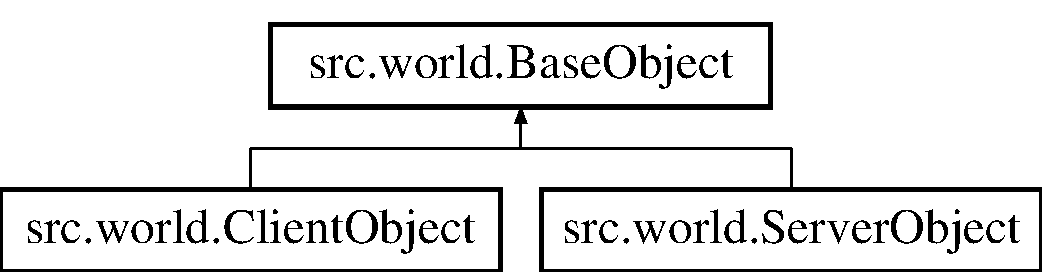
\includegraphics[height=2.000000cm]{classsrc_1_1world_1_1_base_object}
\end{center}
\end{figure}
\subsection*{\-Public \-Member \-Functions}
\begin{DoxyCompactItemize}
\item 
\hypertarget{classsrc_1_1world_1_1_base_object_af9b0564c504dbd3afa84fd94686c23a8}{def {\bfseries \-\_\-\-\_\-init\-\_\-\-\_\-}}\label{classsrc_1_1world_1_1_base_object_af9b0564c504dbd3afa84fd94686c23a8}

\item 
\hypertarget{classsrc_1_1world_1_1_base_object_a9b67f65105eff7e535a8a9e1fa59338c}{def {\bfseries \-\_\-\-\_\-getattr\-\_\-\-\_\-}}\label{classsrc_1_1world_1_1_base_object_a9b67f65105eff7e535a8a9e1fa59338c}

\item 
\hypertarget{classsrc_1_1world_1_1_base_object_a41d299eac2ab4834a7296b7cdebd5c03}{def {\bfseries load}}\label{classsrc_1_1world_1_1_base_object_a41d299eac2ab4834a7296b7cdebd5c03}

\item 
\hypertarget{classsrc_1_1world_1_1_base_object_abb6543d76bbba0b253a9897df843986a}{def {\bfseries context\-Eval}}\label{classsrc_1_1world_1_1_base_object_abb6543d76bbba0b253a9897df843986a}

\end{DoxyCompactItemize}
\subsection*{\-Public \-Attributes}
\begin{DoxyCompactItemize}
\item 
\hypertarget{classsrc_1_1world_1_1_base_object_a61233869acaa51d9beddd921eca8c5ae}{{\bfseries ident}}\label{classsrc_1_1world_1_1_base_object_a61233869acaa51d9beddd921eca8c5ae}

\item 
\hypertarget{classsrc_1_1world_1_1_base_object_a84a88c649a52e017a61ddbdddb733dae}{{\bfseries params}}\label{classsrc_1_1world_1_1_base_object_a84a88c649a52e017a61ddbdddb733dae}

\end{DoxyCompactItemize}
\subsection*{\-Static \-Public \-Attributes}
\begin{DoxyCompactItemize}
\item 
\hypertarget{classsrc_1_1world_1_1_base_object_a25746ae66700933c41eb87f48de16f18}{int {\bfseries ident} = 0}\label{classsrc_1_1world_1_1_base_object_a25746ae66700933c41eb87f48de16f18}

\item 
\hypertarget{classsrc_1_1world_1_1_base_object_a31db5e55de81013c8af360bc8f59f5dd}{dictionary {\bfseries ids} = \{\}}\label{classsrc_1_1world_1_1_base_object_a31db5e55de81013c8af360bc8f59f5dd}

\end{DoxyCompactItemize}


\-The documentation for this class was generated from the following file\-:\begin{DoxyCompactItemize}
\item 
src/world.\-py\end{DoxyCompactItemize}

\hypertarget{classsrc_1_1world_1_1_cell}{\section{src.\-world.\-Cell \-Class \-Reference}
\label{classsrc_1_1world_1_1_cell}\index{src.\-world.\-Cell@{src.\-world.\-Cell}}
}
\subsection*{\-Public \-Member \-Functions}
\begin{DoxyCompactItemize}
\item 
\hypertarget{classsrc_1_1world_1_1_cell_aff5434421d050215d7610716a2da4cba}{def {\bfseries \-\_\-\-\_\-init\-\_\-\-\_\-}}\label{classsrc_1_1world_1_1_cell_aff5434421d050215d7610716a2da4cba}

\end{DoxyCompactItemize}
\subsection*{\-Public \-Attributes}
\begin{DoxyCompactItemize}
\item 
\hypertarget{classsrc_1_1world_1_1_cell_a496918852843c4e7cc880f94aada21ec}{{\bfseries entities}}\label{classsrc_1_1world_1_1_cell_a496918852843c4e7cc880f94aada21ec}

\item 
\hypertarget{classsrc_1_1world_1_1_cell_af304dc75039bf819e4fca168f74ac0c7}{{\bfseries objects}}\label{classsrc_1_1world_1_1_cell_af304dc75039bf819e4fca168f74ac0c7}

\end{DoxyCompactItemize}


\-The documentation for this class was generated from the following file\-:\begin{DoxyCompactItemize}
\item 
src/world.\-py\end{DoxyCompactItemize}

\hypertarget{classsrc_1_1cursescli_1_1_cell_viewer}{\section{src.\-cursescli.\-Cell\-Viewer \-Class \-Reference}
\label{classsrc_1_1cursescli_1_1_cell_viewer}\index{src.\-cursescli.\-Cell\-Viewer@{src.\-cursescli.\-Cell\-Viewer}}
}
\subsection*{\-Public \-Member \-Functions}
\begin{DoxyCompactItemize}
\item 
\hypertarget{classsrc_1_1cursescli_1_1_cell_viewer_aaad19bbe5ea257eebc601041aa687c9f}{def {\bfseries \-\_\-\-\_\-init\-\_\-\-\_\-}}\label{classsrc_1_1cursescli_1_1_cell_viewer_aaad19bbe5ea257eebc601041aa687c9f}

\item 
\hypertarget{classsrc_1_1cursescli_1_1_cell_viewer_a1bddc8a473696ecb4b23135ffefa1f5a}{def {\bfseries display}}\label{classsrc_1_1cursescli_1_1_cell_viewer_a1bddc8a473696ecb4b23135ffefa1f5a}

\end{DoxyCompactItemize}
\subsection*{\-Public \-Attributes}
\begin{DoxyCompactItemize}
\item 
\hypertarget{classsrc_1_1cursescli_1_1_cell_viewer_a8a7327975f255506a724ae857a2a6635}{{\bfseries cell}}\label{classsrc_1_1cursescli_1_1_cell_viewer_a8a7327975f255506a724ae857a2a6635}

\end{DoxyCompactItemize}


\-The documentation for this class was generated from the following file\-:\begin{DoxyCompactItemize}
\item 
src/cursescli.\-py\end{DoxyCompactItemize}

\hypertarget{classsrc_1_1character_1_1_character}{\section{src.\-character.\-Character \-Class \-Reference}
\label{classsrc_1_1character_1_1_character}\index{src.\-character.\-Character@{src.\-character.\-Character}}
}
\subsection*{\-Public \-Member \-Functions}
\begin{DoxyCompactItemize}
\item 
\hypertarget{classsrc_1_1character_1_1_character_a8d23c8f9bc08acd9f50833b99442d2db}{def {\bfseries \-\_\-\-\_\-init\-\_\-\-\_\-}}\label{classsrc_1_1character_1_1_character_a8d23c8f9bc08acd9f50833b99442d2db}

\item 
\hypertarget{classsrc_1_1character_1_1_character_ab245b38ae250a89596fa64e35ba994de}{def {\bfseries render}}\label{classsrc_1_1character_1_1_character_ab245b38ae250a89596fa64e35ba994de}

\item 
\hypertarget{classsrc_1_1character_1_1_character_a38b28a32b53121efaf406d63b9aeb553}{def {\bfseries update}}\label{classsrc_1_1character_1_1_character_a38b28a32b53121efaf406d63b9aeb553}

\item 
\hypertarget{classsrc_1_1character_1_1_character_a08f530ce06eaa3e98893e6187f0d55ff}{def {\bfseries update\-\_\-skin}}\label{classsrc_1_1character_1_1_character_a08f530ce06eaa3e98893e6187f0d55ff}

\item 
\hypertarget{classsrc_1_1character_1_1_character_a42527c58b6594bf86eead5da4d7db7ea}{def {\bfseries zoom}}\label{classsrc_1_1character_1_1_character_a42527c58b6594bf86eead5da4d7db7ea}

\item 
\hypertarget{classsrc_1_1character_1_1_character_a3adec53ea20268070e68f86e1e1ad16d}{def {\bfseries set\-\_\-path}}\label{classsrc_1_1character_1_1_character_a3adec53ea20268070e68f86e1e1ad16d}

\item 
\hypertarget{classsrc_1_1character_1_1_character_aeb893b6369a22260495c4f6c9e7d9456}{def {\bfseries make\-\_\-skin}}\label{classsrc_1_1character_1_1_character_aeb893b6369a22260495c4f6c9e7d9456}

\item 
\hypertarget{classsrc_1_1character_1_1_character_aef87974d3f913d87c34d8eefcf0dd584}{def {\bfseries get\-\_\-cell\-\_\-pos\-\_\-by\-\_\-index}}\label{classsrc_1_1character_1_1_character_aef87974d3f913d87c34d8eefcf0dd584}

\item 
\hypertarget{classsrc_1_1character_1_1_character_a6bdbe8c4ea3b6c68b6a79944ae0a7648}{def {\bfseries move}}\label{classsrc_1_1character_1_1_character_a6bdbe8c4ea3b6c68b6a79944ae0a7648}

\end{DoxyCompactItemize}
\subsection*{\-Public \-Attributes}
\begin{DoxyCompactItemize}
\item 
\hypertarget{classsrc_1_1character_1_1_character_acdbdc52682490096fe1b8a9f8ebf54f1}{{\bfseries skin}}\label{classsrc_1_1character_1_1_character_acdbdc52682490096fe1b8a9f8ebf54f1}

\item 
\hypertarget{classsrc_1_1character_1_1_character_afb3334beb0b06624fd1b650ab7f3f1f1}{{\bfseries name}}\label{classsrc_1_1character_1_1_character_afb3334beb0b06624fd1b650ab7f3f1f1}

\item 
\hypertarget{classsrc_1_1character_1_1_character_aaeb31304eb0ad214589d94c3891a44a3}{{\bfseries action}}\label{classsrc_1_1character_1_1_character_aaeb31304eb0ad214589d94c3891a44a3}

\item 
\hypertarget{classsrc_1_1character_1_1_character_ad317975f0a46245635f2d65705bb0055}{{\bfseries scale}}\label{classsrc_1_1character_1_1_character_ad317975f0a46245635f2d65705bb0055}

\item 
\hypertarget{classsrc_1_1character_1_1_character_a67752e1aa8339b60a05f748857a3e924}{{\bfseries orientation}}\label{classsrc_1_1character_1_1_character_a67752e1aa8339b60a05f748857a3e924}

\item 
\hypertarget{classsrc_1_1character_1_1_character_a3b85117f14fcb32a70770aacae99625c}{{\bfseries image}}\label{classsrc_1_1character_1_1_character_a3b85117f14fcb32a70770aacae99625c}

\item 
\hypertarget{classsrc_1_1character_1_1_character_a80a4c4418fcb5064e33c87b029b41c27}{{\bfseries current\-\_\-image}}\label{classsrc_1_1character_1_1_character_a80a4c4418fcb5064e33c87b029b41c27}

\item 
\hypertarget{classsrc_1_1character_1_1_character_a3b5060e03cad9c58aa4f078b74c959ca}{{\bfseries game\-\_\-frame\-\_\-count}}\label{classsrc_1_1character_1_1_character_a3b5060e03cad9c58aa4f078b74c959ca}

\item 
\hypertarget{classsrc_1_1character_1_1_character_a160bae326cb228a24782601120211c53}{{\bfseries anim\-\_\-frame\-\_\-count}}\label{classsrc_1_1character_1_1_character_a160bae326cb228a24782601120211c53}

\item 
\hypertarget{classsrc_1_1character_1_1_character_a77b7b9a3550d60fea43f3b2173afd6fc}{{\bfseries current\-\_\-cell}}\label{classsrc_1_1character_1_1_character_a77b7b9a3550d60fea43f3b2173afd6fc}

\item 
\hypertarget{classsrc_1_1character_1_1_character_a7d90dc4d446c0b810313cfcdaa0d6aa2}{{\bfseries path}}\label{classsrc_1_1character_1_1_character_a7d90dc4d446c0b810313cfcdaa0d6aa2}

\item 
\hypertarget{classsrc_1_1character_1_1_character_a04b220f94b898f65951cc7506c57d212}{{\bfseries pos\-\_\-offset}}\label{classsrc_1_1character_1_1_character_a04b220f94b898f65951cc7506c57d212}

\end{DoxyCompactItemize}


\-The documentation for this class was generated from the following file\-:\begin{DoxyCompactItemize}
\item 
src/character.\-py\end{DoxyCompactItemize}

\hypertarget{classsrc_1_1chunk_1_1_chunk}{\section{src.\-chunk.\-Chunk \-Class \-Reference}
\label{classsrc_1_1chunk_1_1_chunk}\index{src.\-chunk.\-Chunk@{src.\-chunk.\-Chunk}}
}
\subsection*{\-Public \-Member \-Functions}
\begin{DoxyCompactItemize}
\item 
\hypertarget{classsrc_1_1chunk_1_1_chunk_a204817ea3174038e00cab6d259a4a10f}{def {\bfseries \-\_\-\-\_\-init\-\_\-\-\_\-}}\label{classsrc_1_1chunk_1_1_chunk_a204817ea3174038e00cab6d259a4a10f}

\item 
\hypertarget{classsrc_1_1chunk_1_1_chunk_aaccc5f228bdcef0ace593461d755b068}{def {\bfseries init\-\_\-chunk}}\label{classsrc_1_1chunk_1_1_chunk_aaccc5f228bdcef0ace593461d755b068}

\item 
\hypertarget{classsrc_1_1chunk_1_1_chunk_aea05ade2c559d3aa838103e1326c551c}{def {\bfseries render}}\label{classsrc_1_1chunk_1_1_chunk_aea05ade2c559d3aa838103e1326c551c}

\item 
\hypertarget{classsrc_1_1chunk_1_1_chunk_ab654cd02e8f331610efcc09b64b5326d}{def {\bfseries scale\-\_\-chunk}}\label{classsrc_1_1chunk_1_1_chunk_ab654cd02e8f331610efcc09b64b5326d}

\item 
\hypertarget{classsrc_1_1chunk_1_1_chunk_a13b6d94d12ddeac517d31d32c2b11fe8}{def {\bfseries update}}\label{classsrc_1_1chunk_1_1_chunk_a13b6d94d12ddeac517d31d32c2b11fe8}

\item 
\hypertarget{classsrc_1_1chunk_1_1_chunk_a34dd464aaa303fb791b7d60de9934e32}{def {\bfseries click\-\_\-trigger}}\label{classsrc_1_1chunk_1_1_chunk_a34dd464aaa303fb791b7d60de9934e32}

\item 
\hypertarget{classsrc_1_1chunk_1_1_chunk_ad109d49d69ada1329cf9d89fda50e156}{def {\bfseries set\-\_\-state}}\label{classsrc_1_1chunk_1_1_chunk_ad109d49d69ada1329cf9d89fda50e156}

\item 
\hypertarget{classsrc_1_1chunk_1_1_chunk_a716bc7b600d8a5e83ab39fbba92afb37}{def {\bfseries get\-\_\-state}}\label{classsrc_1_1chunk_1_1_chunk_a716bc7b600d8a5e83ab39fbba92afb37}

\end{DoxyCompactItemize}
\subsection*{\-Public \-Attributes}
\begin{DoxyCompactItemize}
\item 
\hypertarget{classsrc_1_1chunk_1_1_chunk_a82ce0dfa8735315e26aa9c2416a1990f}{{\bfseries index}}\label{classsrc_1_1chunk_1_1_chunk_a82ce0dfa8735315e26aa9c2416a1990f}

\item 
\hypertarget{classsrc_1_1chunk_1_1_chunk_ae7460fc09ed78a35073fcbee362fd632}{{\bfseries cells}}\label{classsrc_1_1chunk_1_1_chunk_ae7460fc09ed78a35073fcbee362fd632}

\item 
\hypertarget{classsrc_1_1chunk_1_1_chunk_aaa7585d6dbe7279632c09e63f01b1852}{{\bfseries g\-\_\-width}}\label{classsrc_1_1chunk_1_1_chunk_aaa7585d6dbe7279632c09e63f01b1852}

\item 
\hypertarget{classsrc_1_1chunk_1_1_chunk_a1983fca8cce8b602d5f913af22f560f3}{{\bfseries g\-\_\-height}}\label{classsrc_1_1chunk_1_1_chunk_a1983fca8cce8b602d5f913af22f560f3}

\item 
\hypertarget{classsrc_1_1chunk_1_1_chunk_a9d81d521c0c57301ed2b63947230cff1}{{\bfseries scale}}\label{classsrc_1_1chunk_1_1_chunk_a9d81d521c0c57301ed2b63947230cff1}

\item 
\hypertarget{classsrc_1_1chunk_1_1_chunk_a5e22e44a7517d38933823b944e467056}{{\bfseries width}}\label{classsrc_1_1chunk_1_1_chunk_a5e22e44a7517d38933823b944e467056}

\item 
\hypertarget{classsrc_1_1chunk_1_1_chunk_a6935c2e39e08c5d5855c87e5cc3fb624}{{\bfseries height}}\label{classsrc_1_1chunk_1_1_chunk_a6935c2e39e08c5d5855c87e5cc3fb624}

\item 
\hypertarget{classsrc_1_1chunk_1_1_chunk_a2d4bb7df9b98984ad3f37988d821dc04}{{\bfseries pos}}\label{classsrc_1_1chunk_1_1_chunk_a2d4bb7df9b98984ad3f37988d821dc04}

\item 
\hypertarget{classsrc_1_1chunk_1_1_chunk_a68ccf275540a2af3c9efcba15713b762}{{\bfseries rect}}\label{classsrc_1_1chunk_1_1_chunk_a68ccf275540a2af3c9efcba15713b762}

\item 
\hypertarget{classsrc_1_1chunk_1_1_chunk_a015e548635e3c3f6b43640852e24a609}{{\bfseries layers}}\label{classsrc_1_1chunk_1_1_chunk_a015e548635e3c3f6b43640852e24a609}

\item 
\hypertarget{classsrc_1_1chunk_1_1_chunk_a6044859819fd7699a93d453c52c16552}{{\bfseries image}}\label{classsrc_1_1chunk_1_1_chunk_a6044859819fd7699a93d453c52c16552}

\end{DoxyCompactItemize}


\-The documentation for this class was generated from the following file\-:\begin{DoxyCompactItemize}
\item 
src/chunk.\-py\end{DoxyCompactItemize}

\hypertarget{classsrc_1_1cache_1_1_chunk_cache}{\section{src.\-cache.\-Chunk\-Cache \-Class \-Reference}
\label{classsrc_1_1cache_1_1_chunk_cache}\index{src.\-cache.\-Chunk\-Cache@{src.\-cache.\-Chunk\-Cache}}
}
\-Inheritance diagram for src.\-cache.\-Chunk\-Cache\-:\begin{figure}[H]
\begin{center}
\leavevmode
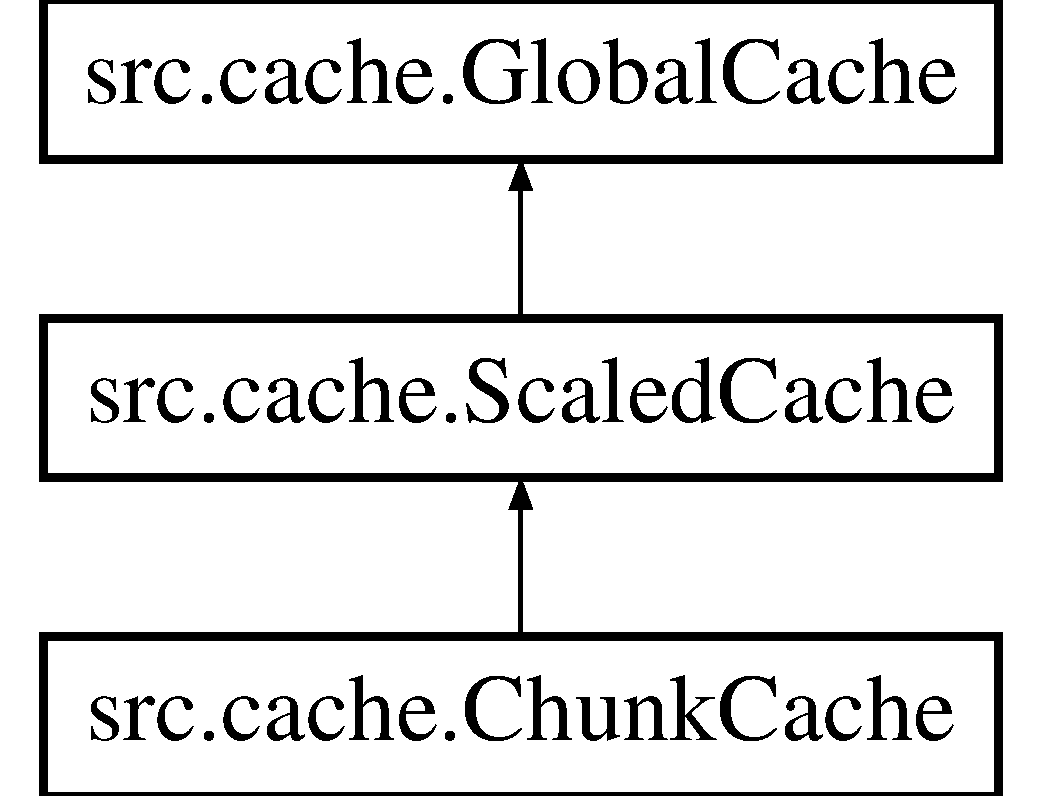
\includegraphics[height=3.000000cm]{classsrc_1_1cache_1_1_chunk_cache}
\end{center}
\end{figure}
\subsection*{\-Public \-Member \-Functions}
\begin{DoxyCompactItemize}
\item 
\hypertarget{classsrc_1_1cache_1_1_chunk_cache_a0aa8988de1687be4dda3acf4d800f761}{def {\bfseries init\-\_\-chunk}}\label{classsrc_1_1cache_1_1_chunk_cache_a0aa8988de1687be4dda3acf4d800f761}

\item 
\hypertarget{classsrc_1_1cache_1_1_chunk_cache_a27271b01addc34ba6d1025a3b07c2327}{def {\bfseries init\-\_\-elts}}\label{classsrc_1_1cache_1_1_chunk_cache_a27271b01addc34ba6d1025a3b07c2327}

\item 
\hypertarget{classsrc_1_1cache_1_1_chunk_cache_a28d77735ab7945fefc93b72dcc327de5}{def {\bfseries init\-\_\-chunks}}\label{classsrc_1_1cache_1_1_chunk_cache_a28d77735ab7945fefc93b72dcc327de5}

\item 
\hypertarget{classsrc_1_1cache_1_1_chunk_cache_afbc38d0fdb2729303afbe947a0f1c94a}{def {\bfseries get\-\_\-chunk}}\label{classsrc_1_1cache_1_1_chunk_cache_afbc38d0fdb2729303afbe947a0f1c94a}

\item 
\hypertarget{classsrc_1_1cache_1_1_chunk_cache_a8d6829cc375aa5c17b4c88390a02baef}{def {\bfseries add\-\_\-scaled}}\label{classsrc_1_1cache_1_1_chunk_cache_a8d6829cc375aa5c17b4c88390a02baef}

\end{DoxyCompactItemize}
\subsection*{\-Static \-Public \-Attributes}
\begin{DoxyCompactItemize}
\item 
\hypertarget{classsrc_1_1cache_1_1_chunk_cache_ad737632ad120595e27c9363c88e5767b}{dictionary {\bfseries cache} = \{\}}\label{classsrc_1_1cache_1_1_chunk_cache_ad737632ad120595e27c9363c88e5767b}

\end{DoxyCompactItemize}


\subsection{\-Detailed \-Description}
\begin{DoxyVerb}
Cache containing instanced chunks. Scale is used for the zoom while
playing the game.
\end{DoxyVerb}
 

\-The documentation for this class was generated from the following file\-:\begin{DoxyCompactItemize}
\item 
src/cache.\-py\end{DoxyCompactItemize}

\hypertarget{classsrc_1_1client_1_1_client}{\section{src.\-client.\-Client \-Class \-Reference}
\label{classsrc_1_1client_1_1_client}\index{src.\-client.\-Client@{src.\-client.\-Client}}
}
\subsection*{\-Public \-Member \-Functions}
\begin{DoxyCompactItemize}
\item 
\hypertarget{classsrc_1_1client_1_1_client_a63e0fbe31d7c47f64ef4e12628f0006f}{def {\bfseries \-\_\-\-\_\-init\-\_\-\-\_\-}}\label{classsrc_1_1client_1_1_client_a63e0fbe31d7c47f64ef4e12628f0006f}

\item 
\hypertarget{classsrc_1_1client_1_1_client_aece67fa18be912de2d7e04840f63d161}{def {\bfseries \-\_\-\-\_\-del\-\_\-\-\_\-}}\label{classsrc_1_1client_1_1_client_aece67fa18be912de2d7e04840f63d161}

\item 
\hypertarget{classsrc_1_1client_1_1_client_a354370a9ad5054293c75e74e79c22280}{def {\bfseries run}}\label{classsrc_1_1client_1_1_client_a354370a9ad5054293c75e74e79c22280}

\item 
\hypertarget{classsrc_1_1client_1_1_client_a6ff2e05841d4fe56bf5d26200763a486}{def {\bfseries frame\-\_\-counter}}\label{classsrc_1_1client_1_1_client_a6ff2e05841d4fe56bf5d26200763a486}

\item 
\hypertarget{classsrc_1_1client_1_1_client_a370da53c7c1f35d0915aea02f5435f29}{def {\bfseries update\-\_\-view}}\label{classsrc_1_1client_1_1_client_a370da53c7c1f35d0915aea02f5435f29}

\item 
\hypertarget{classsrc_1_1client_1_1_client_a4171be6bb67bd1bccfc962070cdd1ac5}{def {\bfseries get\-\_\-conf\-\_\-file}}\label{classsrc_1_1client_1_1_client_a4171be6bb67bd1bccfc962070cdd1ac5}

\item 
\hypertarget{classsrc_1_1client_1_1_client_ae439afc621acd0aa5170187293d876bd}{def {\bfseries get\-\_\-conf}}\label{classsrc_1_1client_1_1_client_ae439afc621acd0aa5170187293d876bd}

\item 
\hypertarget{classsrc_1_1client_1_1_client_aa3c1f7c0648d506a18ef8cc15fa69107}{def {\bfseries init\-\_\-cache}}\label{classsrc_1_1client_1_1_client_aa3c1f7c0648d506a18ef8cc15fa69107}

\item 
\hypertarget{classsrc_1_1client_1_1_client_af341ac55e0b5212451476ea2f69b45e7}{def {\bfseries handle\-Order}}\label{classsrc_1_1client_1_1_client_af341ac55e0b5212451476ea2f69b45e7}

\end{DoxyCompactItemize}
\subsection*{\-Public \-Attributes}
\begin{DoxyCompactItemize}
\item 
\hypertarget{classsrc_1_1client_1_1_client_a22be7470a4f70a1cd0a5c159221e2080}{{\bfseries net}}\label{classsrc_1_1client_1_1_client_a22be7470a4f70a1cd0a5c159221e2080}

\item 
\hypertarget{classsrc_1_1client_1_1_client_af3c8cfb4d4f64c89d220255c940aed00}{{\bfseries screen\-\_\-size}}\label{classsrc_1_1client_1_1_client_af3c8cfb4d4f64c89d220255c940aed00}

\item 
\hypertarget{classsrc_1_1client_1_1_client_a9abfebcb16149fe59da9775af7ea6a8e}{{\bfseries screen}}\label{classsrc_1_1client_1_1_client_a9abfebcb16149fe59da9775af7ea6a8e}

\item 
\hypertarget{classsrc_1_1client_1_1_client_a0c840b0412f44f9220d5c8e7e346527c}{{\bfseries world}}\label{classsrc_1_1client_1_1_client_a0c840b0412f44f9220d5c8e7e346527c}

\item 
\hypertarget{classsrc_1_1client_1_1_client_a78caa6f9fe676a4af8a46c916b1cb413}{{\bfseries interface}}\label{classsrc_1_1client_1_1_client_a78caa6f9fe676a4af8a46c916b1cb413}

\item 
\hypertarget{classsrc_1_1client_1_1_client_ad17d0fea293dd7c11c67a8783530f203}{{\bfseries interactions}}\label{classsrc_1_1client_1_1_client_ad17d0fea293dd7c11c67a8783530f203}

\item 
\hypertarget{classsrc_1_1client_1_1_client_a87fcde6757dca7443d16211dfcb0780f}{{\bfseries perso}}\label{classsrc_1_1client_1_1_client_a87fcde6757dca7443d16211dfcb0780f}

\item 
\hypertarget{classsrc_1_1client_1_1_client_a0c9576fe6e5e83ce95e13bbcbc50c6a2}{{\bfseries order\-Dispatcher}}\label{classsrc_1_1client_1_1_client_a0c9576fe6e5e83ce95e13bbcbc50c6a2}

\item 
\hypertarget{classsrc_1_1client_1_1_client_a3f509c52aeefc5c3b79a8d44abf61921}{{\bfseries background}}\label{classsrc_1_1client_1_1_client_a3f509c52aeefc5c3b79a8d44abf61921}

\item 
\hypertarget{classsrc_1_1client_1_1_client_aa14ee270dca04bd43794ee04d054cbeb}{{\bfseries conf}}\label{classsrc_1_1client_1_1_client_aa14ee270dca04bd43794ee04d054cbeb}

\end{DoxyCompactItemize}


\-The documentation for this class was generated from the following file\-:\begin{DoxyCompactItemize}
\item 
src/client.\-py\end{DoxyCompactItemize}

\hypertarget{classsrc_1_1pygamecli_1_1_client}{}\section{src.\+pygamecli.\+Client Class Reference}
\label{classsrc_1_1pygamecli_1_1_client}\index{src.\+pygamecli.\+Client@{src.\+pygamecli.\+Client}}
\subsection*{Public Member Functions}
\begin{DoxyCompactItemize}
\item 
\hypertarget{classsrc_1_1pygamecli_1_1_client_a026773e6fff92ccb800a1cbe4342829b}{}\label{classsrc_1_1pygamecli_1_1_client_a026773e6fff92ccb800a1cbe4342829b} 
def {\bfseries \+\_\+\+\_\+init\+\_\+\+\_\+} (self, path)
\item 
\hypertarget{classsrc_1_1pygamecli_1_1_client_ac92efdae0937a1aab92800264b8ae9d5}{}\label{classsrc_1_1pygamecli_1_1_client_ac92efdae0937a1aab92800264b8ae9d5} 
def {\bfseries \+\_\+\+\_\+del\+\_\+\+\_\+} (self)
\item 
\hypertarget{classsrc_1_1pygamecli_1_1_client_a7b40cbfdb9c8ef4b3ad0bf77d38ded51}{}\label{classsrc_1_1pygamecli_1_1_client_a7b40cbfdb9c8ef4b3ad0bf77d38ded51} 
def {\bfseries run} (self)
\item 
\hypertarget{classsrc_1_1pygamecli_1_1_client_aed63a1cc434cba703729fbc1644b2e96}{}\label{classsrc_1_1pygamecli_1_1_client_aed63a1cc434cba703729fbc1644b2e96} 
def {\bfseries frame\+\_\+counter} (self, n)
\item 
\hypertarget{classsrc_1_1pygamecli_1_1_client_abdf36b75f4b29e4f2c74d3a6b5144e10}{}\label{classsrc_1_1pygamecli_1_1_client_abdf36b75f4b29e4f2c74d3a6b5144e10} 
def {\bfseries update\+\_\+view} (self, mouse\+\_\+pos, mov\+\_\+speed\+\_\+x, mov\+\_\+speed\+\_\+y, deltat)
\item 
\hypertarget{classsrc_1_1pygamecli_1_1_client_a83d8335f554e9bf57faba2e4ef53e6e9}{}\label{classsrc_1_1pygamecli_1_1_client_a83d8335f554e9bf57faba2e4ef53e6e9} 
def {\bfseries get\+\_\+conf\+\_\+file} (self, path)
\item 
\hypertarget{classsrc_1_1pygamecli_1_1_client_a50c4ff7e216329722138db8fbd37f198}{}\label{classsrc_1_1pygamecli_1_1_client_a50c4ff7e216329722138db8fbd37f198} 
def {\bfseries get\+\_\+conf} (self, conf, type=str)
\item 
\hypertarget{classsrc_1_1pygamecli_1_1_client_a98b0b9df5770463e16b247562d3f15bf}{}\label{classsrc_1_1pygamecli_1_1_client_a98b0b9df5770463e16b247562d3f15bf} 
def {\bfseries init\+\_\+cache} (self)
\item 
\hypertarget{classsrc_1_1pygamecli_1_1_client_a6916abb43b5c9bedeacaaa854f80a9d5}{}\label{classsrc_1_1pygamecli_1_1_client_a6916abb43b5c9bedeacaaa854f80a9d5} 
def {\bfseries handle\+Order} (self, ident, order)
\end{DoxyCompactItemize}
\subsection*{Public Attributes}
\begin{DoxyCompactItemize}
\item 
\hypertarget{classsrc_1_1pygamecli_1_1_client_ac49bab3406de87eeebaf4ea517837174}{}\label{classsrc_1_1pygamecli_1_1_client_ac49bab3406de87eeebaf4ea517837174} 
{\bfseries net}
\item 
\hypertarget{classsrc_1_1pygamecli_1_1_client_a055195a715cdf33f61a51a45576465c4}{}\label{classsrc_1_1pygamecli_1_1_client_a055195a715cdf33f61a51a45576465c4} 
{\bfseries screen\+\_\+size}
\item 
\hypertarget{classsrc_1_1pygamecli_1_1_client_abd74a69bc51c1dbfd1cb9758a616f169}{}\label{classsrc_1_1pygamecli_1_1_client_abd74a69bc51c1dbfd1cb9758a616f169} 
{\bfseries screen}
\item 
\hypertarget{classsrc_1_1pygamecli_1_1_client_a8eedf3dd956cbda87e89c36382bdb7e5}{}\label{classsrc_1_1pygamecli_1_1_client_a8eedf3dd956cbda87e89c36382bdb7e5} 
{\bfseries world}
\item 
\hypertarget{classsrc_1_1pygamecli_1_1_client_a2505375869f2d55692ffd7568f9f8619}{}\label{classsrc_1_1pygamecli_1_1_client_a2505375869f2d55692ffd7568f9f8619} 
{\bfseries interface}
\item 
\hypertarget{classsrc_1_1pygamecli_1_1_client_a381386fd8e7db436983d574b1e570b6b}{}\label{classsrc_1_1pygamecli_1_1_client_a381386fd8e7db436983d574b1e570b6b} 
{\bfseries interactions}
\item 
\hypertarget{classsrc_1_1pygamecli_1_1_client_a2de426209a1bfad65e0a6e0a46303c33}{}\label{classsrc_1_1pygamecli_1_1_client_a2de426209a1bfad65e0a6e0a46303c33} 
{\bfseries perso}
\item 
\hypertarget{classsrc_1_1pygamecli_1_1_client_a1729cd39c4c6d865f6ab55e99d4c1487}{}\label{classsrc_1_1pygamecli_1_1_client_a1729cd39c4c6d865f6ab55e99d4c1487} 
{\bfseries order\+Dispatcher}
\item 
\hypertarget{classsrc_1_1pygamecli_1_1_client_a9ec2972091b06b16117f0baa1d65278b}{}\label{classsrc_1_1pygamecli_1_1_client_a9ec2972091b06b16117f0baa1d65278b} 
{\bfseries background}
\item 
\hypertarget{classsrc_1_1pygamecli_1_1_client_a6b36ebb195e6f899ef039dc5b09bb224}{}\label{classsrc_1_1pygamecli_1_1_client_a6b36ebb195e6f899ef039dc5b09bb224} 
{\bfseries conf}
\end{DoxyCompactItemize}


The documentation for this class was generated from the following file\+:\begin{DoxyCompactItemize}
\item 
src/pygamecli.\+py\end{DoxyCompactItemize}

\hypertarget{classsrc_1_1cursescli_1_1_curses}{\section{src.\-cursescli.\-Curses \-Class \-Reference}
\label{classsrc_1_1cursescli_1_1_curses}\index{src.\-cursescli.\-Curses@{src.\-cursescli.\-Curses}}
}


\-Inherits \-Interface.

\subsection*{\-Public \-Member \-Functions}
\begin{DoxyCompactItemize}
\item 
\hypertarget{classsrc_1_1cursescli_1_1_curses_a0d7e4dc4ed49cdae37b923ab263c3336}{def {\bfseries \-\_\-\-\_\-init\-\_\-\-\_\-}}\label{classsrc_1_1cursescli_1_1_curses_a0d7e4dc4ed49cdae37b923ab263c3336}

\item 
\hypertarget{classsrc_1_1cursescli_1_1_curses_a39cd591bbf83f7f8b3d5ce187d9eb0ef}{def {\bfseries repaint}}\label{classsrc_1_1cursescli_1_1_curses_a39cd591bbf83f7f8b3d5ce187d9eb0ef}

\item 
\hypertarget{classsrc_1_1cursescli_1_1_curses_aa5b522eb03efec0f8357035e64b7ed98}{def {\bfseries end}}\label{classsrc_1_1cursescli_1_1_curses_aa5b522eb03efec0f8357035e64b7ed98}

\item 
\hypertarget{classsrc_1_1cursescli_1_1_curses_acfd11653f75e6ef128877ac8f8422fdf}{def {\bfseries get\-Event}}\label{classsrc_1_1cursescli_1_1_curses_acfd11653f75e6ef128877ac8f8422fdf}

\end{DoxyCompactItemize}
\subsection*{\-Public \-Attributes}
\begin{DoxyCompactItemize}
\item 
\hypertarget{classsrc_1_1cursescli_1_1_curses_aaede7b9ca804d5dbb9b62fb262010f67}{{\bfseries win}}\label{classsrc_1_1cursescli_1_1_curses_aaede7b9ca804d5dbb9b62fb262010f67}

\item 
\hypertarget{classsrc_1_1cursescli_1_1_curses_a339a2a3993480f3e87f69af13c8cd826}{{\bfseries mv}}\label{classsrc_1_1cursescli_1_1_curses_a339a2a3993480f3e87f69af13c8cd826}

\end{DoxyCompactItemize}


\subsection{\-Detailed \-Description}
\begin{DoxyVerb}ncurses-based UI \end{DoxyVerb}
 

\-The documentation for this class was generated from the following file\-:\begin{DoxyCompactItemize}
\item 
src/cursescli.\-py\end{DoxyCompactItemize}

\hypertarget{classsrc_1_1world_1_1_entity}{\section{src.\-world.\-Entity \-Class \-Reference}
\label{classsrc_1_1world_1_1_entity}\index{src.\-world.\-Entity@{src.\-world.\-Entity}}
}
\subsection*{\-Public \-Member \-Functions}
\begin{DoxyCompactItemize}
\item 
\hypertarget{classsrc_1_1world_1_1_entity_a4a2c20fa15aa06f416b783bdd8969a70}{def {\bfseries \-\_\-\-\_\-init\-\_\-\-\_\-}}\label{classsrc_1_1world_1_1_entity_a4a2c20fa15aa06f416b783bdd8969a70}

\end{DoxyCompactItemize}
\subsection*{\-Public \-Attributes}
\begin{DoxyCompactItemize}
\item 
\hypertarget{classsrc_1_1world_1_1_entity_aa2aed1efbc5157f11890fe04f45980b5}{{\bfseries quests}}\label{classsrc_1_1world_1_1_entity_aa2aed1efbc5157f11890fe04f45980b5}

\item 
\hypertarget{classsrc_1_1world_1_1_entity_a22798645d6cc02ddb409797677f51f5f}{{\bfseries inventory}}\label{classsrc_1_1world_1_1_entity_a22798645d6cc02ddb409797677f51f5f}

\end{DoxyCompactItemize}


\-The documentation for this class was generated from the following file\-:\begin{DoxyCompactItemize}
\item 
src/world.\-py\end{DoxyCompactItemize}

\hypertarget{classsrc_1_1cache_1_1_global_cache}{}\section{src.\+cache.\+Global\+Cache Class Reference}
\label{classsrc_1_1cache_1_1_global_cache}\index{src.\+cache.\+Global\+Cache@{src.\+cache.\+Global\+Cache}}
Inheritance diagram for src.\+cache.\+Global\+Cache\+:\begin{figure}[H]
\begin{center}
\leavevmode
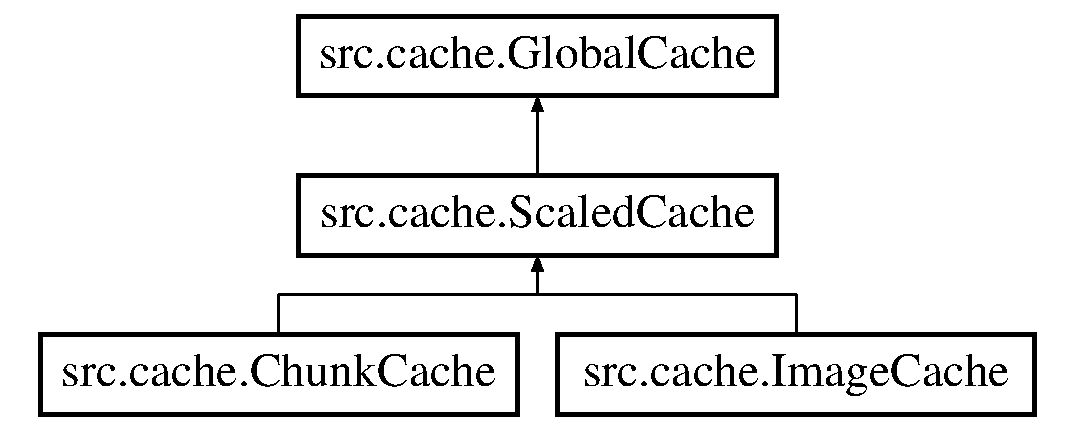
\includegraphics[height=3.000000cm]{classsrc_1_1cache_1_1_global_cache}
\end{center}
\end{figure}
\subsection*{Public Member Functions}
\begin{DoxyCompactItemize}
\item 
\hypertarget{classsrc_1_1cache_1_1_global_cache_aa95fa30f33a7cb2e0a6c7935b90e706c}{}\label{classsrc_1_1cache_1_1_global_cache_aa95fa30f33a7cb2e0a6c7935b90e706c} 
def {\bfseries \+\_\+\+\_\+init\+\_\+\+\_\+} (self)
\item 
\hypertarget{classsrc_1_1cache_1_1_global_cache_a8a2bbb4469040976a555f3c373b7322a}{}\label{classsrc_1_1cache_1_1_global_cache_a8a2bbb4469040976a555f3c373b7322a} 
def {\bfseries set} (cls, key, value)
\item 
\hypertarget{classsrc_1_1cache_1_1_global_cache_a5a8544f65eee5d496052c2f4eb30cba5}{}\label{classsrc_1_1cache_1_1_global_cache_a5a8544f65eee5d496052c2f4eb30cba5} 
def {\bfseries get} (cls, key)
\item 
\hypertarget{classsrc_1_1cache_1_1_global_cache_a093c5f07b870abef862e1e76bf861abc}{}\label{classsrc_1_1cache_1_1_global_cache_a093c5f07b870abef862e1e76bf861abc} 
def {\bfseries clear} (cls)
\item 
\hypertarget{classsrc_1_1cache_1_1_global_cache_abeaa23d23d60a6e91815b8298b064ec2}{}\label{classsrc_1_1cache_1_1_global_cache_abeaa23d23d60a6e91815b8298b064ec2} 
def {\bfseries keys} (cls)
\item 
\hypertarget{classsrc_1_1cache_1_1_global_cache_a62b2e681ac8bbd62f5fd11306ed5f96e}{}\label{classsrc_1_1cache_1_1_global_cache_a62b2e681ac8bbd62f5fd11306ed5f96e} 
def {\bfseries show} (cls)
\end{DoxyCompactItemize}
\subsection*{Public Attributes}
\begin{DoxyCompactItemize}
\item 
\hypertarget{classsrc_1_1cache_1_1_global_cache_a1ccbd28f4abef4193400d308a2b0df23}{}\label{classsrc_1_1cache_1_1_global_cache_a1ccbd28f4abef4193400d308a2b0df23} 
{\bfseries cache}
\end{DoxyCompactItemize}


\subsection{Detailed Description}
\begin{DoxyVerb}A generic cache (key, value) association for objects.
\end{DoxyVerb}
 

The documentation for this class was generated from the following file\+:\begin{DoxyCompactItemize}
\item 
src/cache.\+py\end{DoxyCompactItemize}

\hypertarget{classsrc_1_1cache_1_1_image_cache}{\section{src.\-cache.\-Image\-Cache \-Class \-Reference}
\label{classsrc_1_1cache_1_1_image_cache}\index{src.\-cache.\-Image\-Cache@{src.\-cache.\-Image\-Cache}}
}
\-Inheritance diagram for src.\-cache.\-Image\-Cache\-:\begin{figure}[H]
\begin{center}
\leavevmode
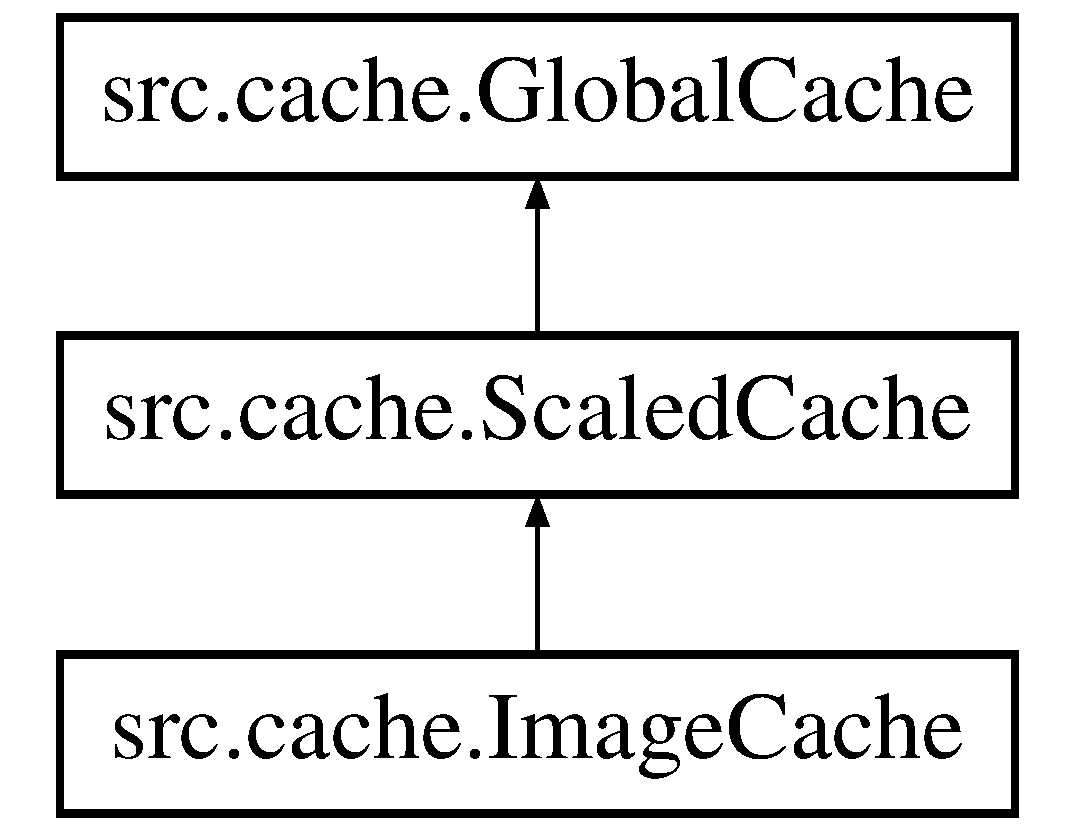
\includegraphics[height=3.000000cm]{classsrc_1_1cache_1_1_image_cache}
\end{center}
\end{figure}
\subsection*{\-Public \-Member \-Functions}
\begin{DoxyCompactItemize}
\item 
\hypertarget{classsrc_1_1cache_1_1_image_cache_a4c9f29d5205ed27f97b076e19c16c054}{def {\bfseries init\-\_\-image\-\_\-from\-\_\-file}}\label{classsrc_1_1cache_1_1_image_cache_a4c9f29d5205ed27f97b076e19c16c054}

\item 
\hypertarget{classsrc_1_1cache_1_1_image_cache_a366263eba8f84df37fe6e3a7d5ddbf89}{def {\bfseries init\-\_\-image\-\_\-from\-\_\-surface}}\label{classsrc_1_1cache_1_1_image_cache_a366263eba8f84df37fe6e3a7d5ddbf89}

\item 
\hypertarget{classsrc_1_1cache_1_1_image_cache_a3af2b0b8c88860d2cca143441fd90227}{def {\bfseries get\-\_\-image}}\label{classsrc_1_1cache_1_1_image_cache_a3af2b0b8c88860d2cca143441fd90227}

\item 
\hypertarget{classsrc_1_1cache_1_1_image_cache_a751bf8d48a4389c93039436f9aca0452}{def {\bfseries init\-\_\-elts}}\label{classsrc_1_1cache_1_1_image_cache_a751bf8d48a4389c93039436f9aca0452}

\item 
\hypertarget{classsrc_1_1cache_1_1_image_cache_a987c2d16f67eb59dc94ddc2f49dcf613}{def {\bfseries init\-\_\-images}}\label{classsrc_1_1cache_1_1_image_cache_a987c2d16f67eb59dc94ddc2f49dcf613}

\item 
\hypertarget{classsrc_1_1cache_1_1_image_cache_a4c4f0b82c9585d9499a3aa197f9376c1}{def {\bfseries add\-\_\-scaled}}\label{classsrc_1_1cache_1_1_image_cache_a4c4f0b82c9585d9499a3aa197f9376c1}

\end{DoxyCompactItemize}
\subsection*{\-Static \-Public \-Attributes}
\begin{DoxyCompactItemize}
\item 
\hypertarget{classsrc_1_1cache_1_1_image_cache_abf4f360706061a9524b39be34cdf711e}{dictionary {\bfseries cache} = \{\}}\label{classsrc_1_1cache_1_1_image_cache_abf4f360706061a9524b39be34cdf711e}

\end{DoxyCompactItemize}


\-The documentation for this class was generated from the following file\-:\begin{DoxyCompactItemize}
\item 
src/cache.\-py\end{DoxyCompactItemize}

\hypertarget{classsrc_1_1interactions_1_1_interaction}{\section{src.\-interactions.\-Interaction \-Class \-Reference}
\label{classsrc_1_1interactions_1_1_interaction}\index{src.\-interactions.\-Interaction@{src.\-interactions.\-Interaction}}
}
\subsection*{\-Public \-Member \-Functions}
\begin{DoxyCompactItemize}
\item 
\hypertarget{classsrc_1_1interactions_1_1_interaction_a97a1759e258a88c8b6e31e1afde852b9}{def {\bfseries \-\_\-\-\_\-init\-\_\-\-\_\-}}\label{classsrc_1_1interactions_1_1_interaction_a97a1759e258a88c8b6e31e1afde852b9}

\item 
\hypertarget{classsrc_1_1interactions_1_1_interaction_a96ccab0afe3e927e94f5c39fe1b59cfc}{def {\bfseries load}}\label{classsrc_1_1interactions_1_1_interaction_a96ccab0afe3e927e94f5c39fe1b59cfc}

\end{DoxyCompactItemize}
\subsection*{\-Public \-Attributes}
\begin{DoxyCompactItemize}
\item 
\hypertarget{classsrc_1_1interactions_1_1_interaction_ad577ad6550f3bad2cf45192bcdd2d659}{{\bfseries target}}\label{classsrc_1_1interactions_1_1_interaction_ad577ad6550f3bad2cf45192bcdd2d659}

\item 
\hypertarget{classsrc_1_1interactions_1_1_interaction_a455988c49a2625914d11e97e0b1b9285}{{\bfseries type}}\label{classsrc_1_1interactions_1_1_interaction_a455988c49a2625914d11e97e0b1b9285}

\item 
\hypertarget{classsrc_1_1interactions_1_1_interaction_ae0115c68842371d5c28d85f2234c9d4b}{{\bfseries key}}\label{classsrc_1_1interactions_1_1_interaction_ae0115c68842371d5c28d85f2234c9d4b}

\item 
\hypertarget{classsrc_1_1interactions_1_1_interaction_aec1ad3a52431ab38496a0ce83a21b7f1}{{\bfseries event}}\label{classsrc_1_1interactions_1_1_interaction_aec1ad3a52431ab38496a0ce83a21b7f1}

\end{DoxyCompactItemize}


\-The documentation for this class was generated from the following file\-:\begin{DoxyCompactItemize}
\item 
src/interactions.\-py\end{DoxyCompactItemize}

\hypertarget{classsrc_1_1print_world_1_1_interface}{}\section{src.\+print\+World.\+Interface Class Reference}
\label{classsrc_1_1print_world_1_1_interface}\index{src.\+print\+World.\+Interface@{src.\+print\+World.\+Interface}}
Inheritance diagram for src.\+print\+World.\+Interface\+:\begin{figure}[H]
\begin{center}
\leavevmode
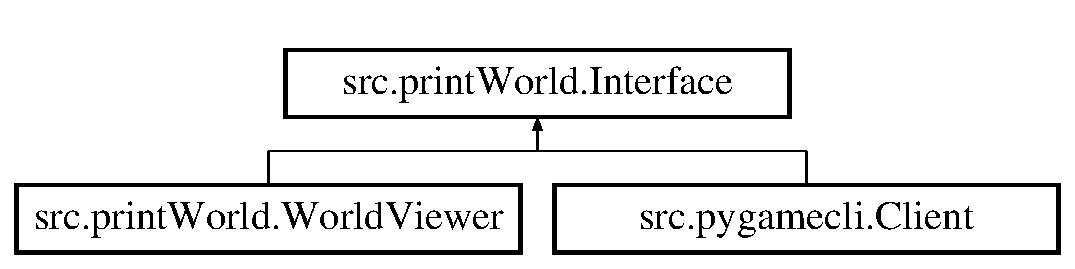
\includegraphics[height=2.000000cm]{classsrc_1_1print_world_1_1_interface}
\end{center}
\end{figure}


The documentation for this class was generated from the following file\+:\begin{DoxyCompactItemize}
\item 
src/print\+World.\+py\end{DoxyCompactItemize}

\hypertarget{classsrc_1_1interface_1_1_interface}{}\section{src.\+interface.\+Interface Class Reference}
\label{classsrc_1_1interface_1_1_interface}\index{src.\+interface.\+Interface@{src.\+interface.\+Interface}}
Inheritance diagram for src.\+interface.\+Interface\+:\begin{figure}[H]
\begin{center}
\leavevmode
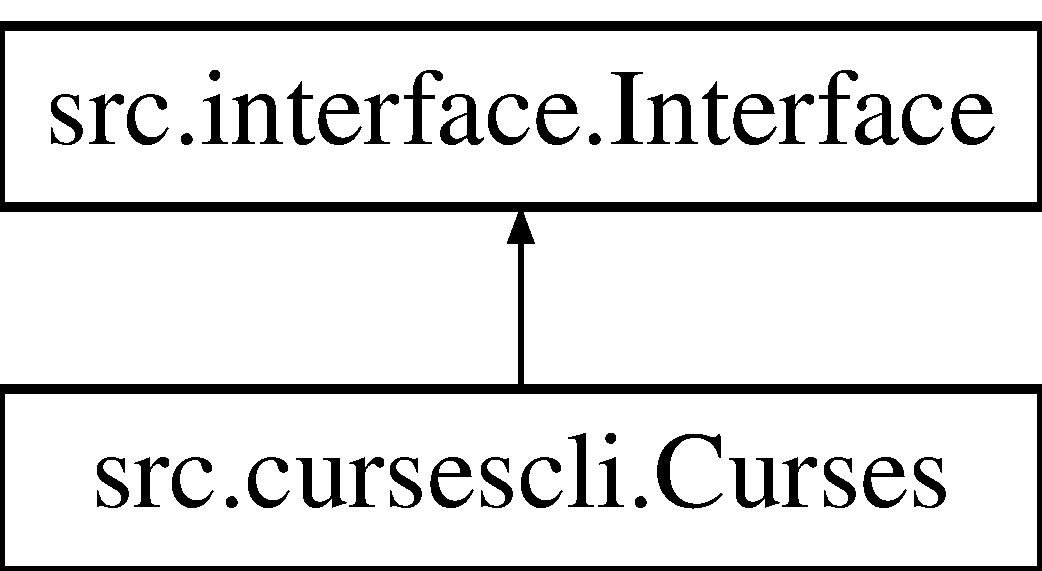
\includegraphics[height=2.000000cm]{classsrc_1_1interface_1_1_interface}
\end{center}
\end{figure}
\subsection*{Public Member Functions}
\begin{DoxyCompactItemize}
\item 
\hypertarget{classsrc_1_1interface_1_1_interface_afd85ca0e9d4d7241eb7cc3fc278e382e}{}\label{classsrc_1_1interface_1_1_interface_afd85ca0e9d4d7241eb7cc3fc278e382e} 
def {\bfseries \+\_\+\+\_\+init\+\_\+\+\_\+} (self, w)
\item 
\hypertarget{classsrc_1_1interface_1_1_interface_a208bd509d61790c767cf2e2e244251e6}{}\label{classsrc_1_1interface_1_1_interface_a208bd509d61790c767cf2e2e244251e6} 
def {\bfseries update} (self)
\item 
\hypertarget{classsrc_1_1interface_1_1_interface_a568bdcd1f15799b98e7fddd66e53538a}{}\label{classsrc_1_1interface_1_1_interface_a568bdcd1f15799b98e7fddd66e53538a} 
def {\bfseries repaint} (self)
\item 
\hypertarget{classsrc_1_1interface_1_1_interface_a36f0c0435e8999755a96095c5b0d3e91}{}\label{classsrc_1_1interface_1_1_interface_a36f0c0435e8999755a96095c5b0d3e91} 
def {\bfseries init} (self)
\item 
\hypertarget{classsrc_1_1interface_1_1_interface_a7220f63d562c2a8eb934f8a7233fd326}{}\label{classsrc_1_1interface_1_1_interface_a7220f63d562c2a8eb934f8a7233fd326} 
def {\bfseries end} (self)
\item 
\hypertarget{classsrc_1_1interface_1_1_interface_aae4bd8e4081596c5dec5013aed5c8ac0}{}\label{classsrc_1_1interface_1_1_interface_aae4bd8e4081596c5dec5013aed5c8ac0} 
def {\bfseries get\+Event} (self)
\end{DoxyCompactItemize}
\subsection*{Public Attributes}
\begin{DoxyCompactItemize}
\item 
\hypertarget{classsrc_1_1interface_1_1_interface_ae3f574913c0f42acfe8869b6f1b53f97}{}\label{classsrc_1_1interface_1_1_interface_ae3f574913c0f42acfe8869b6f1b53f97} 
{\bfseries world}
\item 
\hypertarget{classsrc_1_1interface_1_1_interface_a6841bfb944d99e869903790a57cd57ab}{}\label{classsrc_1_1interface_1_1_interface_a6841bfb944d99e869903790a57cd57ab} 
{\bfseries last\+Update}
\end{DoxyCompactItemize}


\subsection{Detailed Description}
\begin{DoxyVerb}UI base-class, can be used as a dummy interface \end{DoxyVerb}
 

The documentation for this class was generated from the following file\+:\begin{DoxyCompactItemize}
\item 
src/interface.\+py\end{DoxyCompactItemize}

\hypertarget{classsrc_1_1layer_1_1_layer}{}\section{src.\+layer.\+Layer Class Reference}
\label{classsrc_1_1layer_1_1_layer}\index{src.\+layer.\+Layer@{src.\+layer.\+Layer}}
Inheritance diagram for src.\+layer.\+Layer\+:\begin{figure}[H]
\begin{center}
\leavevmode
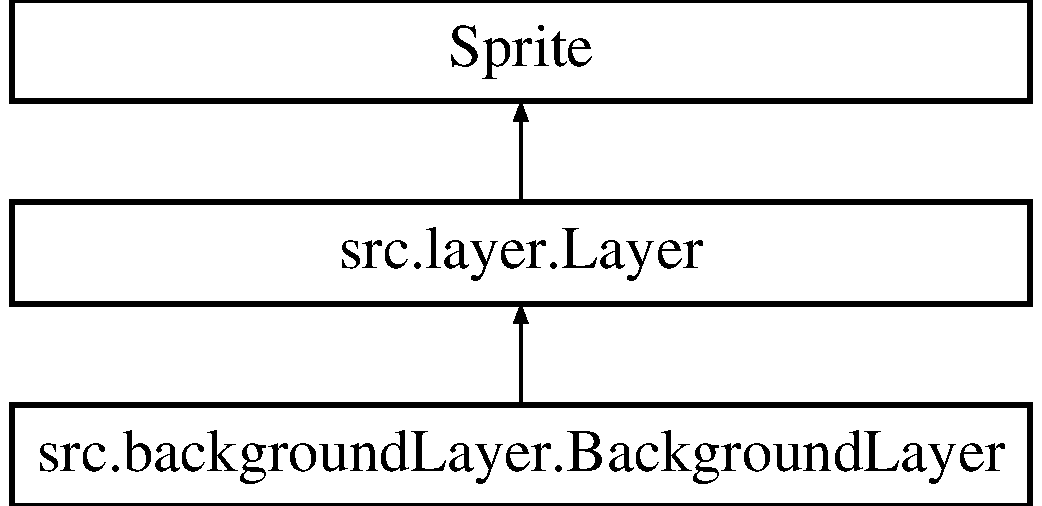
\includegraphics[height=3.000000cm]{classsrc_1_1layer_1_1_layer}
\end{center}
\end{figure}
\subsection*{Public Member Functions}
\begin{DoxyCompactItemize}
\item 
\hypertarget{classsrc_1_1layer_1_1_layer_afb0f95173b44d2cd9942a3bec2b84eeb}{}\label{classsrc_1_1layer_1_1_layer_afb0f95173b44d2cd9942a3bec2b84eeb} 
def {\bfseries \+\_\+\+\_\+init\+\_\+\+\_\+} (self, size)
\item 
\hypertarget{classsrc_1_1layer_1_1_layer_a78a4e2da87ec9a61fe566359ace3d67b}{}\label{classsrc_1_1layer_1_1_layer_a78a4e2da87ec9a61fe566359ace3d67b} 
def {\bfseries render} (self, surf)
\item 
\hypertarget{classsrc_1_1layer_1_1_layer_a6f780023058a52954127d05226d167f7}{}\label{classsrc_1_1layer_1_1_layer_a6f780023058a52954127d05226d167f7} 
def {\bfseries update} (self)
\item 
\hypertarget{classsrc_1_1layer_1_1_layer_acb009d1cb2cbb276f3e1d880dc766190}{}\label{classsrc_1_1layer_1_1_layer_acb009d1cb2cbb276f3e1d880dc766190} 
def {\bfseries get\+\_\+cell\+\_\+pos} (self, c\+\_\+line, c\+\_\+col, size\+\_\+image)
\item 
def \hyperlink{classsrc_1_1layer_1_1_layer_a6d99c2cef696b679bbc26f4307b21427}{make\+\_\+grid} (self, img\+\_\+set, cell\+\_\+ids)
\end{DoxyCompactItemize}
\subsection*{Public Attributes}
\begin{DoxyCompactItemize}
\item 
\hypertarget{classsrc_1_1layer_1_1_layer_a9b228afc78fa22b3aed57cc426b53956}{}\label{classsrc_1_1layer_1_1_layer_a9b228afc78fa22b3aed57cc426b53956} 
{\bfseries cells}
\item 
\hypertarget{classsrc_1_1layer_1_1_layer_af2a57c9ef96b6855db07ec0cd3dca58e}{}\label{classsrc_1_1layer_1_1_layer_af2a57c9ef96b6855db07ec0cd3dca58e} 
{\bfseries g\+\_\+width}
\item 
\hypertarget{classsrc_1_1layer_1_1_layer_a627dbe4baccfa8b611aa6286677b3d80}{}\label{classsrc_1_1layer_1_1_layer_a627dbe4baccfa8b611aa6286677b3d80} 
{\bfseries g\+\_\+height}
\item 
\hypertarget{classsrc_1_1layer_1_1_layer_ab51fb62aca8248f38b3f3dfe7206fe87}{}\label{classsrc_1_1layer_1_1_layer_ab51fb62aca8248f38b3f3dfe7206fe87} 
{\bfseries size}
\end{DoxyCompactItemize}


\subsection{Detailed Description}
\begin{DoxyVerb}A abstract class defining a layer of the display (ex. background) \end{DoxyVerb}
 

\subsection{Member Function Documentation}
\hypertarget{classsrc_1_1layer_1_1_layer_a6d99c2cef696b679bbc26f4307b21427}{}\label{classsrc_1_1layer_1_1_layer_a6d99c2cef696b679bbc26f4307b21427} 
\index{src\+::layer\+::\+Layer@{src\+::layer\+::\+Layer}!make\+\_\+grid@{make\+\_\+grid}}
\index{make\+\_\+grid@{make\+\_\+grid}!src\+::layer\+::\+Layer@{src\+::layer\+::\+Layer}}
\subsubsection{\texorpdfstring{make\+\_\+grid()}{make\_grid()}}
{\footnotesize\ttfamily def src.\+layer.\+Layer.\+make\+\_\+grid (\begin{DoxyParamCaption}\item[{}]{self,  }\item[{}]{img\+\_\+set,  }\item[{}]{cell\+\_\+ids }\end{DoxyParamCaption})}

\begin{DoxyVerb}Build the grid that will be drawn by Pygame. Img_set is a list
of (id/type, filename) specifying the files to load for each type
of cell and cell_ids is the type for each cell.
\end{DoxyVerb}
 

The documentation for this class was generated from the following file\+:\begin{DoxyCompactItemize}
\item 
src/layer.\+py\end{DoxyCompactItemize}

\hypertarget{classsrc_1_1world_1_1_map}{\section{src.\-world.\-Map \-Class \-Reference}
\label{classsrc_1_1world_1_1_map}\index{src.\-world.\-Map@{src.\-world.\-Map}}
}
\subsection*{\-Public \-Member \-Functions}
\begin{DoxyCompactItemize}
\item 
\hypertarget{classsrc_1_1world_1_1_map_ad9d8e58739ea61b490d37743810432ec}{def {\bfseries \-\_\-\-\_\-init\-\_\-\-\_\-}}\label{classsrc_1_1world_1_1_map_ad9d8e58739ea61b490d37743810432ec}

\item 
def \hyperlink{classsrc_1_1world_1_1_map_a44caa8c25ebb963130a5a70255d94299}{fill}
\end{DoxyCompactItemize}
\subsection*{\-Public \-Attributes}
\begin{DoxyCompactItemize}
\item 
\hypertarget{classsrc_1_1world_1_1_map_a5efc29105a33cfeabf12c5fe7c199a5c}{{\bfseries cells}}\label{classsrc_1_1world_1_1_map_a5efc29105a33cfeabf12c5fe7c199a5c}

\item 
\hypertarget{classsrc_1_1world_1_1_map_a89ebb1d9301db6f4399c64c2e82708c7}{{\bfseries cells\-Grid}}\label{classsrc_1_1world_1_1_map_a89ebb1d9301db6f4399c64c2e82708c7}

\end{DoxyCompactItemize}


\subsection{\-Member \-Function \-Documentation}
\hypertarget{classsrc_1_1world_1_1_map_a44caa8c25ebb963130a5a70255d94299}{\index{src\-::world\-::\-Map@{src\-::world\-::\-Map}!fill@{fill}}
\index{fill@{fill}!src::world::Map@{src\-::world\-::\-Map}}
\subsubsection[{fill}]{\setlength{\rightskip}{0pt plus 5cm}def {\bf src.\-world.\-Map.\-fill} (
\begin{DoxyParamCaption}
\item[{}]{self}
\end{DoxyParamCaption}
)}}\label{classsrc_1_1world_1_1_map_a44caa8c25ebb963130a5a70255d94299}
\begin{DoxyVerb}Complète les cases par défaut \end{DoxyVerb}
 

\-The documentation for this class was generated from the following file\-:\begin{DoxyCompactItemize}
\item 
src/world.\-py\end{DoxyCompactItemize}

\hypertarget{classsrc_1_1cursescli_1_1_map_viewer}{\section{src.\-cursescli.\-Map\-Viewer \-Class \-Reference}
\label{classsrc_1_1cursescli_1_1_map_viewer}\index{src.\-cursescli.\-Map\-Viewer@{src.\-cursescli.\-Map\-Viewer}}
}
\subsection*{\-Public \-Member \-Functions}
\begin{DoxyCompactItemize}
\item 
\hypertarget{classsrc_1_1cursescli_1_1_map_viewer_adb6b4b3785a77d27d5572ad0dce523cd}{def {\bfseries \-\_\-\-\_\-init\-\_\-\-\_\-}}\label{classsrc_1_1cursescli_1_1_map_viewer_adb6b4b3785a77d27d5572ad0dce523cd}

\item 
\hypertarget{classsrc_1_1cursescli_1_1_map_viewer_a718d614417fb7004b3ffde1ca750ac8c}{def {\bfseries display}}\label{classsrc_1_1cursescli_1_1_map_viewer_a718d614417fb7004b3ffde1ca750ac8c}

\end{DoxyCompactItemize}
\subsection*{\-Public \-Attributes}
\begin{DoxyCompactItemize}
\item 
\hypertarget{classsrc_1_1cursescli_1_1_map_viewer_ac3f7f8b0aa940244e7a7b13b40c8b410}{{\bfseries map}}\label{classsrc_1_1cursescli_1_1_map_viewer_ac3f7f8b0aa940244e7a7b13b40c8b410}

\item 
\hypertarget{classsrc_1_1cursescli_1_1_map_viewer_a866adc09259481040308ff887910987c}{{\bfseries world}}\label{classsrc_1_1cursescli_1_1_map_viewer_a866adc09259481040308ff887910987c}

\item 
\hypertarget{classsrc_1_1cursescli_1_1_map_viewer_a7beea5f1784ce6cbc23533294afd1e58}{{\bfseries cell\-Views}}\label{classsrc_1_1cursescli_1_1_map_viewer_a7beea5f1784ce6cbc23533294afd1e58}

\end{DoxyCompactItemize}


\-The documentation for this class was generated from the following file\-:\begin{DoxyCompactItemize}
\item 
src/cursescli.\-py\end{DoxyCompactItemize}

\hypertarget{classsrc_1_1map_1_1_map_viewer}{\section{src.\-map.\-Map\-Viewer \-Class \-Reference}
\label{classsrc_1_1map_1_1_map_viewer}\index{src.\-map.\-Map\-Viewer@{src.\-map.\-Map\-Viewer}}
}
\subsection*{\-Public \-Member \-Functions}
\begin{DoxyCompactItemize}
\item 
\hypertarget{classsrc_1_1map_1_1_map_viewer_a8997ec02710136f8bd6ebf59c63da281}{def {\bfseries \-\_\-\-\_\-init\-\_\-\-\_\-}}\label{classsrc_1_1map_1_1_map_viewer_a8997ec02710136f8bd6ebf59c63da281}

\item 
\hypertarget{classsrc_1_1map_1_1_map_viewer_a07a318fee6ef7bb30d191734e80a08ac}{def {\bfseries load\-\_\-chunks}}\label{classsrc_1_1map_1_1_map_viewer_a07a318fee6ef7bb30d191734e80a08ac}

\item 
\hypertarget{classsrc_1_1map_1_1_map_viewer_ac4f4367839d4e069c704342d75a5b763}{def {\bfseries make\-\_\-walkables}}\label{classsrc_1_1map_1_1_map_viewer_ac4f4367839d4e069c704342d75a5b763}

\item 
\hypertarget{classsrc_1_1map_1_1_map_viewer_a06296998c8b4ec64c1bfe1c5d16c0ca1}{def {\bfseries zoom}}\label{classsrc_1_1map_1_1_map_viewer_a06296998c8b4ec64c1bfe1c5d16c0ca1}

\item 
\hypertarget{classsrc_1_1map_1_1_map_viewer_ae8e7465bf22e8b6c624c57610d568091}{def {\bfseries move}}\label{classsrc_1_1map_1_1_map_viewer_ae8e7465bf22e8b6c624c57610d568091}

\item 
\hypertarget{classsrc_1_1map_1_1_map_viewer_a8b6327cbebaac59b59a07c8d48994f39}{def {\bfseries render}}\label{classsrc_1_1map_1_1_map_viewer_a8b6327cbebaac59b59a07c8d48994f39}

\item 
def \hyperlink{classsrc_1_1map_1_1_map_viewer_a79cdbef74bdb68268f83b1f6cac622e8}{neighbors\-\_\-chunk}
\item 
\hypertarget{classsrc_1_1map_1_1_map_viewer_a98ed63282992c7a07e1920ba58e54148}{def {\bfseries onscreen\-\_\-chunks}}\label{classsrc_1_1map_1_1_map_viewer_a98ed63282992c7a07e1920ba58e54148}

\item 
\hypertarget{classsrc_1_1map_1_1_map_viewer_a41a58673346c7d7dbe04fcb2e9b494e3}{def {\bfseries update}}\label{classsrc_1_1map_1_1_map_viewer_a41a58673346c7d7dbe04fcb2e9b494e3}

\item 
\hypertarget{classsrc_1_1map_1_1_map_viewer_aaf52a4bbcfc8d5aa47506948e106c3de}{def {\bfseries propagate\-\_\-trigger}}\label{classsrc_1_1map_1_1_map_viewer_aaf52a4bbcfc8d5aa47506948e106c3de}

\item 
\hypertarget{classsrc_1_1map_1_1_map_viewer_a2e8a049f5b60798b117530bbbee0bb09}{def {\bfseries compute\-\_\-path}}\label{classsrc_1_1map_1_1_map_viewer_a2e8a049f5b60798b117530bbbee0bb09}

\item 
\hypertarget{classsrc_1_1map_1_1_map_viewer_aacea41d6ff85a99e4dd286b303c35c3b}{def {\bfseries load\-\_\-bg}}\label{classsrc_1_1map_1_1_map_viewer_aacea41d6ff85a99e4dd286b303c35c3b}

\end{DoxyCompactItemize}
\subsection*{\-Public \-Attributes}
\begin{DoxyCompactItemize}
\item 
\hypertarget{classsrc_1_1map_1_1_map_viewer_a7ddc42713b0a5147cd23bf159163c43a}{{\bfseries map}}\label{classsrc_1_1map_1_1_map_viewer_a7ddc42713b0a5147cd23bf159163c43a}

\item 
\hypertarget{classsrc_1_1map_1_1_map_viewer_a9c0b186ce3fb12c2a68a614e0a0255db}{{\bfseries world}}\label{classsrc_1_1map_1_1_map_viewer_a9c0b186ce3fb12c2a68a614e0a0255db}

\item 
\hypertarget{classsrc_1_1map_1_1_map_viewer_a5ec08ee96a88c1a6403ca54bf40b9ba9}{{\bfseries scale}}\label{classsrc_1_1map_1_1_map_viewer_a5ec08ee96a88c1a6403ca54bf40b9ba9}

\item 
\hypertarget{classsrc_1_1map_1_1_map_viewer_af3d3e0f89f118bce440c7cc8c8665777}{{\bfseries cm\-\_\-height}}\label{classsrc_1_1map_1_1_map_viewer_af3d3e0f89f118bce440c7cc8c8665777}

\item 
\hypertarget{classsrc_1_1map_1_1_map_viewer_a192bf9aea058941bf26c186b7df9c6f4}{{\bfseries width}}\label{classsrc_1_1map_1_1_map_viewer_a192bf9aea058941bf26c186b7df9c6f4}

\item 
\hypertarget{classsrc_1_1map_1_1_map_viewer_a2482715662b085064aec22c59bfc06b0}{{\bfseries height}}\label{classsrc_1_1map_1_1_map_viewer_a2482715662b085064aec22c59bfc06b0}

\item 
\hypertarget{classsrc_1_1map_1_1_map_viewer_af781403ec69ef33b2e1a3cb4eac834e5}{{\bfseries walkables\-Graph}}\label{classsrc_1_1map_1_1_map_viewer_af781403ec69ef33b2e1a3cb4eac834e5}

\item 
\hypertarget{classsrc_1_1map_1_1_map_viewer_a084bd729a289751d881444ca5154192b}{{\bfseries current\-\_\-chunk}}\label{classsrc_1_1map_1_1_map_viewer_a084bd729a289751d881444ca5154192b}

\item 
\hypertarget{classsrc_1_1map_1_1_map_viewer_a78602046c0d74ec7e969f6558216ea68}{{\bfseries pos\-\_\-offset}}\label{classsrc_1_1map_1_1_map_viewer_a78602046c0d74ec7e969f6558216ea68}

\item 
\hypertarget{classsrc_1_1map_1_1_map_viewer_aeb83e9eb17ada2dc3f46ba3bd21eda47}{{\bfseries chunk\-\_\-pos}}\label{classsrc_1_1map_1_1_map_viewer_aeb83e9eb17ada2dc3f46ba3bd21eda47}

\item 
\hypertarget{classsrc_1_1map_1_1_map_viewer_a235b396649899f2075c63ee695b4513f}{{\bfseries chunks\-\_\-state}}\label{classsrc_1_1map_1_1_map_viewer_a235b396649899f2075c63ee695b4513f}

\end{DoxyCompactItemize}


\subsection{\-Member \-Function \-Documentation}
\hypertarget{classsrc_1_1map_1_1_map_viewer_a79cdbef74bdb68268f83b1f6cac622e8}{\index{src\-::map\-::\-Map\-Viewer@{src\-::map\-::\-Map\-Viewer}!neighbors\-\_\-chunk@{neighbors\-\_\-chunk}}
\index{neighbors\-\_\-chunk@{neighbors\-\_\-chunk}!src::map::MapViewer@{src\-::map\-::\-Map\-Viewer}}
\subsubsection[{neighbors\-\_\-chunk}]{\setlength{\rightskip}{0pt plus 5cm}def {\bf src.\-map.\-Map\-Viewer.\-neighbors\-\_\-chunk} (
\begin{DoxyParamCaption}
\item[{}]{self, }
\item[{}]{chunk}
\end{DoxyParamCaption}
)}}\label{classsrc_1_1map_1_1_map_viewer_a79cdbef74bdb68268f83b1f6cac622e8}
\begin{DoxyVerb}Returns indexes of the neighbors of chunk and index of chunk \end{DoxyVerb}
 

\-The documentation for this class was generated from the following file\-:\begin{DoxyCompactItemize}
\item 
src/map.\-py\end{DoxyCompactItemize}

\hypertarget{classsrc_1_1network_1_1_network_client}{}\section{src.\+network.\+Network\+Client Class Reference}
\label{classsrc_1_1network_1_1_network_client}\index{src.\+network.\+Network\+Client@{src.\+network.\+Network\+Client}}
\subsection*{Public Member Functions}
\begin{DoxyCompactItemize}
\item 
\hypertarget{classsrc_1_1network_1_1_network_client_ac916d4beefd5d85ecf1c9f868778ba0a}{}\label{classsrc_1_1network_1_1_network_client_ac916d4beefd5d85ecf1c9f868778ba0a} 
def {\bfseries \+\_\+\+\_\+init\+\_\+\+\_\+} (self, handle)
\item 
def \hyperlink{classsrc_1_1network_1_1_network_client_a284788cf59342797e77659bbf1f01077}{ask\+Entity} (self, ent)
\item 
\hypertarget{classsrc_1_1network_1_1_network_client_aff658527c0a9eddaa94566b59d2bc280}{}\label{classsrc_1_1network_1_1_network_client_aff658527c0a9eddaa94566b59d2bc280} 
def {\bfseries connect} (self)
\item 
def \hyperlink{classsrc_1_1network_1_1_network_client_ab93bfbf5db5822ecb056aa4ed70b9378}{run} (self)
\item 
\hypertarget{classsrc_1_1network_1_1_network_client_aea7fd43ebd9030cfed6133ec45f07104}{}\label{classsrc_1_1network_1_1_network_client_aea7fd43ebd9030cfed6133ec45f07104} 
def {\bfseries send} (self, m)
\item 
def \hyperlink{classsrc_1_1network_1_1_network_client_a5464ebb5a065e4234703c93bf664f228}{send\+Event} (self, obj, event)
\item 
\hypertarget{classsrc_1_1network_1_1_network_client_aceb091634efd3b262be5d9879b91637a}{}\label{classsrc_1_1network_1_1_network_client_aceb091634efd3b262be5d9879b91637a} 
def {\bfseries kill} (self)
\end{DoxyCompactItemize}
\subsection*{Public Attributes}
\begin{DoxyCompactItemize}
\item 
\hypertarget{classsrc_1_1network_1_1_network_client_ae54784438c7710b1adc53f1bdeb9a2e5}{}\label{classsrc_1_1network_1_1_network_client_ae54784438c7710b1adc53f1bdeb9a2e5} 
{\bfseries handle}
\item 
\hypertarget{classsrc_1_1network_1_1_network_client_a0c5773f7b2800d9d34fb4e248602851c}{}\label{classsrc_1_1network_1_1_network_client_a0c5773f7b2800d9d34fb4e248602851c} 
{\bfseries alive}
\item 
\hypertarget{classsrc_1_1network_1_1_network_client_ade3948e9b9eeabf9d0d1555c19b26f2d}{}\label{classsrc_1_1network_1_1_network_client_ade3948e9b9eeabf9d0d1555c19b26f2d} 
{\bfseries writer}
\end{DoxyCompactItemize}


\subsection{Detailed Description}
\begin{DoxyVerb}This class manages the network activities of the client.
It allows the client to send messages (describing events) to the server.
\end{DoxyVerb}
 

\subsection{Member Function Documentation}
\hypertarget{classsrc_1_1network_1_1_network_client_a284788cf59342797e77659bbf1f01077}{}\label{classsrc_1_1network_1_1_network_client_a284788cf59342797e77659bbf1f01077} 
\index{src\+::network\+::\+Network\+Client@{src\+::network\+::\+Network\+Client}!ask\+Entity@{ask\+Entity}}
\index{ask\+Entity@{ask\+Entity}!src\+::network\+::\+Network\+Client@{src\+::network\+::\+Network\+Client}}
\subsubsection{\texorpdfstring{ask\+Entity()}{askEntity()}}
{\footnotesize\ttfamily def src.\+network.\+Network\+Client.\+ask\+Entity (\begin{DoxyParamCaption}\item[{}]{self,  }\item[{}]{ent }\end{DoxyParamCaption})}

\begin{DoxyVerb}Ask for an entity \end{DoxyVerb}
 \hypertarget{classsrc_1_1network_1_1_network_client_ab93bfbf5db5822ecb056aa4ed70b9378}{}\label{classsrc_1_1network_1_1_network_client_ab93bfbf5db5822ecb056aa4ed70b9378} 
\index{src\+::network\+::\+Network\+Client@{src\+::network\+::\+Network\+Client}!run@{run}}
\index{run@{run}!src\+::network\+::\+Network\+Client@{src\+::network\+::\+Network\+Client}}
\subsubsection{\texorpdfstring{run()}{run()}}
{\footnotesize\ttfamily def src.\+network.\+Network\+Client.\+run (\begin{DoxyParamCaption}\item[{}]{self }\end{DoxyParamCaption})}

\begin{DoxyVerb}Main loop of the client's network task.  After connecting the socket
to the server, wait for orders and handle them immediately until
connection ends.
\end{DoxyVerb}
 \hypertarget{classsrc_1_1network_1_1_network_client_a5464ebb5a065e4234703c93bf664f228}{}\label{classsrc_1_1network_1_1_network_client_a5464ebb5a065e4234703c93bf664f228} 
\index{src\+::network\+::\+Network\+Client@{src\+::network\+::\+Network\+Client}!send\+Event@{send\+Event}}
\index{send\+Event@{send\+Event}!src\+::network\+::\+Network\+Client@{src\+::network\+::\+Network\+Client}}
\subsubsection{\texorpdfstring{send\+Event()}{sendEvent()}}
{\footnotesize\ttfamily def src.\+network.\+Network\+Client.\+send\+Event (\begin{DoxyParamCaption}\item[{}]{self,  }\item[{}]{obj,  }\item[{}]{event }\end{DoxyParamCaption})}

\begin{DoxyVerb}Send an event to the server in a formatted way, specifying the id
of the object to affect.
\end{DoxyVerb}
 

The documentation for this class was generated from the following file\+:\begin{DoxyCompactItemize}
\item 
src/network.\+py\end{DoxyCompactItemize}

\hypertarget{classsrc_1_1networkudp_1_1_network_client}{}\section{src.\+networkudp.\+Network\+Client Class Reference}
\label{classsrc_1_1networkudp_1_1_network_client}\index{src.\+networkudp.\+Network\+Client@{src.\+networkudp.\+Network\+Client}}
Inheritance diagram for src.\+networkudp.\+Network\+Client\+:\begin{figure}[H]
\begin{center}
\leavevmode
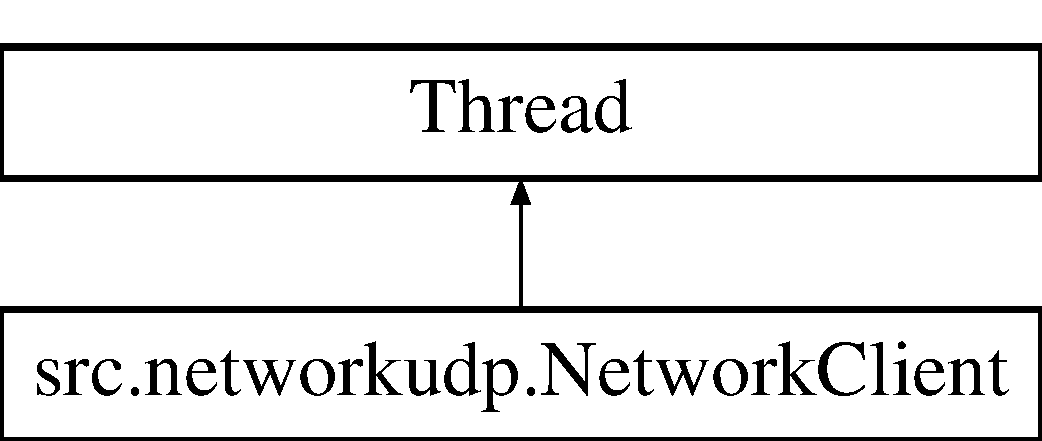
\includegraphics[height=2.000000cm]{classsrc_1_1networkudp_1_1_network_client}
\end{center}
\end{figure}
\subsection*{Public Member Functions}
\begin{DoxyCompactItemize}
\item 
\hypertarget{classsrc_1_1networkudp_1_1_network_client_a30b40ebc598599f405162c742d8ba886}{}\label{classsrc_1_1networkudp_1_1_network_client_a30b40ebc598599f405162c742d8ba886} 
def {\bfseries \+\_\+\+\_\+init\+\_\+\+\_\+} (self, handle)
\item 
\hypertarget{classsrc_1_1networkudp_1_1_network_client_ae3e8fe50b963e813333bfb30069327e3}{}\label{classsrc_1_1networkudp_1_1_network_client_ae3e8fe50b963e813333bfb30069327e3} 
def {\bfseries run} (self)
\item 
\hypertarget{classsrc_1_1networkudp_1_1_network_client_aa1041d91d3544565d54b81f199335c8c}{}\label{classsrc_1_1networkudp_1_1_network_client_aa1041d91d3544565d54b81f199335c8c} 
def {\bfseries send} (self, m)
\item 
\hypertarget{classsrc_1_1networkudp_1_1_network_client_a184a0dc3819bd1927cd99c6b1d6fe645}{}\label{classsrc_1_1networkudp_1_1_network_client_a184a0dc3819bd1927cd99c6b1d6fe645} 
def {\bfseries send\+Event} (self, obj, eve)
\item 
\hypertarget{classsrc_1_1networkudp_1_1_network_client_a38b3e8ed3fa5e7a018de0ceece270e68}{}\label{classsrc_1_1networkudp_1_1_network_client_a38b3e8ed3fa5e7a018de0ceece270e68} 
def {\bfseries kill} (self)
\end{DoxyCompactItemize}
\subsection*{Public Attributes}
\begin{DoxyCompactItemize}
\item 
\hypertarget{classsrc_1_1networkudp_1_1_network_client_ae3a6e8899b864601d8d1c43092ffbc1d}{}\label{classsrc_1_1networkudp_1_1_network_client_ae3a6e8899b864601d8d1c43092ffbc1d} 
{\bfseries handle}
\item 
\hypertarget{classsrc_1_1networkudp_1_1_network_client_ab331a8c61f46f49e2fc0beab52986ace}{}\label{classsrc_1_1networkudp_1_1_network_client_ab331a8c61f46f49e2fc0beab52986ace} 
{\bfseries soc}
\item 
\hypertarget{classsrc_1_1networkudp_1_1_network_client_a445685f7d171bc82c3ec6f11a2320ef3}{}\label{classsrc_1_1networkudp_1_1_network_client_a445685f7d171bc82c3ec6f11a2320ef3} 
{\bfseries alive}
\end{DoxyCompactItemize}


The documentation for this class was generated from the following file\+:\begin{DoxyCompactItemize}
\item 
src/networkudp.\+py\end{DoxyCompactItemize}

\hypertarget{classsrc_1_1network_1_1_network_server}{\section{src.\-network.\-Network\-Server \-Class \-Reference}
\label{classsrc_1_1network_1_1_network_server}\index{src.\-network.\-Network\-Server@{src.\-network.\-Network\-Server}}
}


\-Inherits \-Thread.

\subsection*{\-Public \-Member \-Functions}
\begin{DoxyCompactItemize}
\item 
\hypertarget{classsrc_1_1network_1_1_network_server_a039e381f87c229e9158c452edb57b8a3}{def {\bfseries \-\_\-\-\_\-init\-\_\-\-\_\-}}\label{classsrc_1_1network_1_1_network_server_a039e381f87c229e9158c452edb57b8a3}

\item 
\hypertarget{classsrc_1_1network_1_1_network_server_af334f8d7eed6eca8a8ba7088945634a9}{def {\bfseries wait\-For\-Clients}}\label{classsrc_1_1network_1_1_network_server_af334f8d7eed6eca8a8ba7088945634a9}

\item 
\hypertarget{classsrc_1_1network_1_1_network_server_ad0dba462246e4f49d69ce4b5395389e1}{def {\bfseries run}}\label{classsrc_1_1network_1_1_network_server_ad0dba462246e4f49d69ce4b5395389e1}

\item 
\hypertarget{classsrc_1_1network_1_1_network_server_afdb13f3f3e49a452518553d7c980772f}{def {\bfseries send\-Order}}\label{classsrc_1_1network_1_1_network_server_afdb13f3f3e49a452518553d7c980772f}

\item 
\hypertarget{classsrc_1_1network_1_1_network_server_a03dc0456c8bf224b47531f171dbecf69}{def {\bfseries broadcast}}\label{classsrc_1_1network_1_1_network_server_a03dc0456c8bf224b47531f171dbecf69}

\item 
\hypertarget{classsrc_1_1network_1_1_network_server_a617ffd6ccce5e6c852c50ab39d779588}{def {\bfseries kill}}\label{classsrc_1_1network_1_1_network_server_a617ffd6ccce5e6c852c50ab39d779588}

\end{DoxyCompactItemize}
\subsection*{\-Public \-Attributes}
\begin{DoxyCompactItemize}
\item 
\hypertarget{classsrc_1_1network_1_1_network_server_a69b93e1961b39b8f938935cc180777be}{{\bfseries handle}}\label{classsrc_1_1network_1_1_network_server_a69b93e1961b39b8f938935cc180777be}

\item 
\hypertarget{classsrc_1_1network_1_1_network_server_ad6f4eb2f6a295b6850dab572f0db4292}{{\bfseries soc}}\label{classsrc_1_1network_1_1_network_server_ad6f4eb2f6a295b6850dab572f0db4292}

\item 
\hypertarget{classsrc_1_1network_1_1_network_server_ab384a6e8eca2b22a0d3aef7bb3a8f843}{{\bfseries alive}}\label{classsrc_1_1network_1_1_network_server_ab384a6e8eca2b22a0d3aef7bb3a8f843}

\item 
\hypertarget{classsrc_1_1network_1_1_network_server_ac9dadc4baef43efefe4ceab0e44e4d4c}{{\bfseries co}}\label{classsrc_1_1network_1_1_network_server_ac9dadc4baef43efefe4ceab0e44e4d4c}

\end{DoxyCompactItemize}


\-The documentation for this class was generated from the following file\-:\begin{DoxyCompactItemize}
\item 
src/network.\-py\end{DoxyCompactItemize}

\hypertarget{classsrc_1_1networkudp_1_1_network_server}{\section{src.\-networkudp.\-Network\-Server \-Class \-Reference}
\label{classsrc_1_1networkudp_1_1_network_server}\index{src.\-networkudp.\-Network\-Server@{src.\-networkudp.\-Network\-Server}}
}


\-Inherits \-Thread.

\subsection*{\-Public \-Member \-Functions}
\begin{DoxyCompactItemize}
\item 
\hypertarget{classsrc_1_1networkudp_1_1_network_server_a0f2e7b248ad9f5bae9ebe4274291e703}{def {\bfseries \-\_\-\-\_\-init\-\_\-\-\_\-}}\label{classsrc_1_1networkudp_1_1_network_server_a0f2e7b248ad9f5bae9ebe4274291e703}

\item 
\hypertarget{classsrc_1_1networkudp_1_1_network_server_aef027ba8a2e09b28ba6cde2110a914df}{def {\bfseries wait\-For\-Clients}}\label{classsrc_1_1networkudp_1_1_network_server_aef027ba8a2e09b28ba6cde2110a914df}

\item 
\hypertarget{classsrc_1_1networkudp_1_1_network_server_a535af8cc05c677b0d17cd6151b3b92e3}{def {\bfseries run}}\label{classsrc_1_1networkudp_1_1_network_server_a535af8cc05c677b0d17cd6151b3b92e3}

\item 
\hypertarget{classsrc_1_1networkudp_1_1_network_server_aa94aa32c52003e6e4f00d8e6137ad72c}{def {\bfseries send\-Order}}\label{classsrc_1_1networkudp_1_1_network_server_aa94aa32c52003e6e4f00d8e6137ad72c}

\item 
\hypertarget{classsrc_1_1networkudp_1_1_network_server_a5574b9156e04bec0d1d5eec428f4bc61}{def {\bfseries broadcast}}\label{classsrc_1_1networkudp_1_1_network_server_a5574b9156e04bec0d1d5eec428f4bc61}

\item 
\hypertarget{classsrc_1_1networkudp_1_1_network_server_ae48e706f92a60de9cef98bd281552f85}{def {\bfseries kill}}\label{classsrc_1_1networkudp_1_1_network_server_ae48e706f92a60de9cef98bd281552f85}

\end{DoxyCompactItemize}
\subsection*{\-Public \-Attributes}
\begin{DoxyCompactItemize}
\item 
\hypertarget{classsrc_1_1networkudp_1_1_network_server_a7aebdf344b0392f532ff00483d556f21}{{\bfseries handle}}\label{classsrc_1_1networkudp_1_1_network_server_a7aebdf344b0392f532ff00483d556f21}

\item 
\hypertarget{classsrc_1_1networkudp_1_1_network_server_a99617b6eb70a2bc48fd90af30a40d177}{{\bfseries soc}}\label{classsrc_1_1networkudp_1_1_network_server_a99617b6eb70a2bc48fd90af30a40d177}

\item 
\hypertarget{classsrc_1_1networkudp_1_1_network_server_a1529d8df546f6a9d816368009fb79690}{{\bfseries alive}}\label{classsrc_1_1networkudp_1_1_network_server_a1529d8df546f6a9d816368009fb79690}

\item 
\hypertarget{classsrc_1_1networkudp_1_1_network_server_a034c43c4b6226da3cdec505b0957db57}{{\bfseries addr}}\label{classsrc_1_1networkudp_1_1_network_server_a034c43c4b6226da3cdec505b0957db57}

\end{DoxyCompactItemize}


\-The documentation for this class was generated from the following file\-:\begin{DoxyCompactItemize}
\item 
src/networkudp.\-py\end{DoxyCompactItemize}

\hypertarget{classsrc_1_1world_1_1_object_type}{\section{src.\-world.\-Object\-Type \-Class \-Reference}
\label{classsrc_1_1world_1_1_object_type}\index{src.\-world.\-Object\-Type@{src.\-world.\-Object\-Type}}
}
\subsection*{\-Public \-Member \-Functions}
\begin{DoxyCompactItemize}
\item 
\hypertarget{classsrc_1_1world_1_1_object_type_ac8a8a5e2f760dc7ad47a122c2f81260a}{def {\bfseries \-\_\-\-\_\-init\-\_\-\-\_\-}}\label{classsrc_1_1world_1_1_object_type_ac8a8a5e2f760dc7ad47a122c2f81260a}

\item 
def \hyperlink{classsrc_1_1world_1_1_object_type_ad802e763a2a37cccc20b98e1d6b35fb6}{create}
\item 
\hypertarget{classsrc_1_1world_1_1_object_type_a08d5b8ddd6761e8ac32f5c0bda5f9eae}{def {\bfseries \-\_\-\-\_\-str\-\_\-\-\_\-}}\label{classsrc_1_1world_1_1_object_type_a08d5b8ddd6761e8ac32f5c0bda5f9eae}

\end{DoxyCompactItemize}
\subsection*{\-Public \-Attributes}
\begin{DoxyCompactItemize}
\item 
\hypertarget{classsrc_1_1world_1_1_object_type_a9a72a17c18cf9dcf1e078609ca81aa3a}{{\bfseries type}}\label{classsrc_1_1world_1_1_object_type_a9a72a17c18cf9dcf1e078609ca81aa3a}

\end{DoxyCompactItemize}


\subsection{\-Detailed \-Description}
\begin{DoxyVerb}Les types d'objets (au sens informatique) \end{DoxyVerb}
 

\subsection{\-Member \-Function \-Documentation}
\hypertarget{classsrc_1_1world_1_1_object_type_ad802e763a2a37cccc20b98e1d6b35fb6}{\index{src\-::world\-::\-Object\-Type@{src\-::world\-::\-Object\-Type}!create@{create}}
\index{create@{create}!src::world::ObjectType@{src\-::world\-::\-Object\-Type}}
\subsubsection[{create}]{\setlength{\rightskip}{0pt plus 5cm}def {\bf src.\-world.\-Object\-Type.\-create} (
\begin{DoxyParamCaption}
\item[{}]{self}
\end{DoxyParamCaption}
)}}\label{classsrc_1_1world_1_1_object_type_ad802e763a2a37cccc20b98e1d6b35fb6}
\begin{DoxyVerb}Instanticiation d'un objet à partir du type \end{DoxyVerb}
 

\-The documentation for this class was generated from the following file\-:\begin{DoxyCompactItemize}
\item 
src/world.\-py\end{DoxyCompactItemize}

\hypertarget{classsrc_1_1orders_1_1_order}{\section{src.\-orders.\-Order \-Class \-Reference}
\label{classsrc_1_1orders_1_1_order}\index{src.\-orders.\-Order@{src.\-orders.\-Order}}
}
\subsection*{\-Public \-Member \-Functions}
\begin{DoxyCompactItemize}
\item 
\hypertarget{classsrc_1_1orders_1_1_order_ac1fbb5b5c8f81d1e203e478eec1a29fb}{def {\bfseries \-\_\-\-\_\-init\-\_\-\-\_\-}}\label{classsrc_1_1orders_1_1_order_ac1fbb5b5c8f81d1e203e478eec1a29fb}

\item 
\hypertarget{classsrc_1_1orders_1_1_order_a64e9fbf0310096a6532057f1b9d05c5a}{def {\bfseries \-\_\-\-\_\-getattr\-\_\-\-\_\-}}\label{classsrc_1_1orders_1_1_order_a64e9fbf0310096a6532057f1b9d05c5a}

\item 
\hypertarget{classsrc_1_1orders_1_1_order_abde48245d90eebc476ddf27ebc2c73d1}{def {\bfseries \-\_\-\-\_\-setattr\-\_\-\-\_\-}}\label{classsrc_1_1orders_1_1_order_abde48245d90eebc476ddf27ebc2c73d1}

\item 
\hypertarget{classsrc_1_1orders_1_1_order_a97a7c5d09e2acccc49fb015e518738b8}{def {\bfseries copy}}\label{classsrc_1_1orders_1_1_order_a97a7c5d09e2acccc49fb015e518738b8}

\item 
def \hyperlink{classsrc_1_1orders_1_1_order_a04d6d02084832b8e7e0d977cb333eab1}{load}
\item 
def \hyperlink{classsrc_1_1orders_1_1_order_aa48ef819154770b19b524b534283c183}{to\-Bytes}
\item 
def \hyperlink{classsrc_1_1orders_1_1_order_a727cb258b2f5d787d02eec14523f9f6b}{from\-Bytes}
\end{DoxyCompactItemize}
\subsection*{\-Public \-Attributes}
\begin{DoxyCompactItemize}
\item 
\hypertarget{classsrc_1_1orders_1_1_order_aa520998f666493616c058406413cc7dc}{{\bfseries type}}\label{classsrc_1_1orders_1_1_order_aa520998f666493616c058406413cc7dc}

\item 
\hypertarget{classsrc_1_1orders_1_1_order_a0b890f5803ed3e710da29b4d612967dc}{{\bfseries args}}\label{classsrc_1_1orders_1_1_order_a0b890f5803ed3e710da29b4d612967dc}

\end{DoxyCompactItemize}
\subsection*{\-Static \-Public \-Attributes}
\begin{DoxyCompactItemize}
\item 
\hypertarget{classsrc_1_1orders_1_1_order_aa15ac874941c1dd31e60be3ba4a89e91}{list {\bfseries params} = \mbox{[}\-None\mbox{]}}\label{classsrc_1_1orders_1_1_order_aa15ac874941c1dd31e60be3ba4a89e91}

\end{DoxyCompactItemize}


\subsection{\-Detailed \-Description}
\begin{DoxyVerb}Représente une modification à apporter au monde \end{DoxyVerb}
 

\subsection{\-Member \-Function \-Documentation}
\hypertarget{classsrc_1_1orders_1_1_order_a727cb258b2f5d787d02eec14523f9f6b}{\index{src\-::orders\-::\-Order@{src\-::orders\-::\-Order}!from\-Bytes@{from\-Bytes}}
\index{from\-Bytes@{from\-Bytes}!src::orders::Order@{src\-::orders\-::\-Order}}
\subsubsection[{from\-Bytes}]{\setlength{\rightskip}{0pt plus 5cm}def {\bf src.\-orders.\-Order.\-from\-Bytes} (
\begin{DoxyParamCaption}
\item[{}]{self, }
\item[{}]{b}
\end{DoxyParamCaption}
)}}\label{classsrc_1_1orders_1_1_order_a727cb258b2f5d787d02eec14523f9f6b}
\begin{DoxyVerb}Récupère l'ordre à partir d'un bytes réseau \end{DoxyVerb}
 \hypertarget{classsrc_1_1orders_1_1_order_a04d6d02084832b8e7e0d977cb333eab1}{\index{src\-::orders\-::\-Order@{src\-::orders\-::\-Order}!load@{load}}
\index{load@{load}!src::orders::Order@{src\-::orders\-::\-Order}}
\subsubsection[{load}]{\setlength{\rightskip}{0pt plus 5cm}def {\bf src.\-orders.\-Order.\-load} (
\begin{DoxyParamCaption}
\item[{}]{self, }
\item[{}]{dat, }
\item[{}]{named}
\end{DoxyParamCaption}
)}}\label{classsrc_1_1orders_1_1_order_a04d6d02084832b8e7e0d977cb333eab1}
\begin{DoxyVerb}Initialise l'ordre avec une structure provenant d'un Xml \end{DoxyVerb}
 \hypertarget{classsrc_1_1orders_1_1_order_aa48ef819154770b19b524b534283c183}{\index{src\-::orders\-::\-Order@{src\-::orders\-::\-Order}!to\-Bytes@{to\-Bytes}}
\index{to\-Bytes@{to\-Bytes}!src::orders::Order@{src\-::orders\-::\-Order}}
\subsubsection[{to\-Bytes}]{\setlength{\rightskip}{0pt plus 5cm}def {\bf src.\-orders.\-Order.\-to\-Bytes} (
\begin{DoxyParamCaption}
\item[{}]{self}
\end{DoxyParamCaption}
)}}\label{classsrc_1_1orders_1_1_order_aa48ef819154770b19b524b534283c183}
\begin{DoxyVerb}Bytes pour envoyer l'ordre sur le réseau \end{DoxyVerb}
 

\-The documentation for this class was generated from the following file\-:\begin{DoxyCompactItemize}
\item 
src/orders.\-py\end{DoxyCompactItemize}

\hypertarget{classsrc_1_1orders_1_1_order_dispatcher}{\section{src.\-orders.\-Order\-Dispatcher \-Class \-Reference}
\label{classsrc_1_1orders_1_1_order_dispatcher}\index{src.\-orders.\-Order\-Dispatcher@{src.\-orders.\-Order\-Dispatcher}}
}
\subsection*{\-Public \-Member \-Functions}
\begin{DoxyCompactItemize}
\item 
\hypertarget{classsrc_1_1orders_1_1_order_dispatcher_a72be66c7756e667e0f48da3feb526db8}{def {\bfseries \-\_\-\-\_\-init\-\_\-\-\_\-}}\label{classsrc_1_1orders_1_1_order_dispatcher_a72be66c7756e667e0f48da3feb526db8}

\item 
def \hyperlink{classsrc_1_1orders_1_1_order_dispatcher_af7e1d2ad1021e105f8a810e45163a2a6}{treat}
\end{DoxyCompactItemize}
\subsection*{\-Public \-Attributes}
\begin{DoxyCompactItemize}
\item 
\hypertarget{classsrc_1_1orders_1_1_order_dispatcher_a3e1eb5983064b2b581cfbe29e5d8d4a4}{{\bfseries world}}\label{classsrc_1_1orders_1_1_order_dispatcher_a3e1eb5983064b2b581cfbe29e5d8d4a4}

\item 
\hypertarget{classsrc_1_1orders_1_1_order_dispatcher_af3a628629fdbcc412086c3a2ad36263f}{{\bfseries handle}}\label{classsrc_1_1orders_1_1_order_dispatcher_af3a628629fdbcc412086c3a2ad36263f}

\item 
\hypertarget{classsrc_1_1orders_1_1_order_dispatcher_a874829894f821dcf4229f015dc033773}{{\bfseries timer}}\label{classsrc_1_1orders_1_1_order_dispatcher_a874829894f821dcf4229f015dc033773}

\end{DoxyCompactItemize}


\subsection{\-Detailed \-Description}
\begin{DoxyVerb}Traite les ordres pour le client ou le serveur \end{DoxyVerb}
 

\subsection{\-Member \-Function \-Documentation}
\hypertarget{classsrc_1_1orders_1_1_order_dispatcher_af7e1d2ad1021e105f8a810e45163a2a6}{\index{src\-::orders\-::\-Order\-Dispatcher@{src\-::orders\-::\-Order\-Dispatcher}!treat@{treat}}
\index{treat@{treat}!src::orders::OrderDispatcher@{src\-::orders\-::\-Order\-Dispatcher}}
\subsubsection[{treat}]{\setlength{\rightskip}{0pt plus 5cm}def {\bf src.\-orders.\-Order\-Dispatcher.\-treat} (
\begin{DoxyParamCaption}
\item[{}]{self, }
\item[{}]{emitter, }
\item[{}]{order}
\end{DoxyParamCaption}
)}}\label{classsrc_1_1orders_1_1_order_dispatcher_af7e1d2ad1021e105f8a810e45163a2a6}
\begin{DoxyVerb}Traite un ordre et renvoie l'éventuel ordre à retransmettre \end{DoxyVerb}
 

\-The documentation for this class was generated from the following file\-:\begin{DoxyCompactItemize}
\item 
src/orders.\-py\end{DoxyCompactItemize}

\hypertarget{classsrc_1_1tools_1_1_perf}{\section{src.\-tools.\-Perf \-Class \-Reference}
\label{classsrc_1_1tools_1_1_perf}\index{src.\-tools.\-Perf@{src.\-tools.\-Perf}}
}
\subsection*{\-Public \-Member \-Functions}
\begin{DoxyCompactItemize}
\item 
\hypertarget{classsrc_1_1tools_1_1_perf_ae919d5b427e84955a7b24c50db43215f}{def {\bfseries \-\_\-\-\_\-init\-\_\-\-\_\-}}\label{classsrc_1_1tools_1_1_perf_ae919d5b427e84955a7b24c50db43215f}

\item 
def \hyperlink{classsrc_1_1tools_1_1_perf_a0704b72e2ac5342defa88b5c550021a2}{tic}
\item 
def \hyperlink{classsrc_1_1tools_1_1_perf_a18a53770729072c60b8b7323b09c9d2a}{toc}
\item 
def \hyperlink{classsrc_1_1tools_1_1_perf_a3a93246501e8c3327e8e1a8e2c34e051}{show}
\end{DoxyCompactItemize}
\subsection*{\-Public \-Attributes}
\begin{DoxyCompactItemize}
\item 
\hypertarget{classsrc_1_1tools_1_1_perf_aa643b113c85e3bbb79594f7e891e261c}{{\bfseries num}}\label{classsrc_1_1tools_1_1_perf_aa643b113c85e3bbb79594f7e891e261c}

\item 
\hypertarget{classsrc_1_1tools_1_1_perf_a0ec2cd1d0283f00834da46b00a6fc284}{{\bfseries avg}}\label{classsrc_1_1tools_1_1_perf_a0ec2cd1d0283f00834da46b00a6fc284}

\item 
\hypertarget{classsrc_1_1tools_1_1_perf_a13fa4a0d1c9e7ef999d4870e27fdee07}{{\bfseries min}}\label{classsrc_1_1tools_1_1_perf_a13fa4a0d1c9e7ef999d4870e27fdee07}

\item 
\hypertarget{classsrc_1_1tools_1_1_perf_ae4714b793a290019961788298f7e4353}{{\bfseries max}}\label{classsrc_1_1tools_1_1_perf_ae4714b793a290019961788298f7e4353}

\item 
\hypertarget{classsrc_1_1tools_1_1_perf_a0dc9b6afdeb4e9d14cf3436d8117b5e6}{{\bfseries t}}\label{classsrc_1_1tools_1_1_perf_a0dc9b6afdeb4e9d14cf3436d8117b5e6}

\end{DoxyCompactItemize}


\subsection{\-Detailed \-Description}
\begin{DoxyVerb}Calcule les performances d'un morceau de code \end{DoxyVerb}
 

\subsection{\-Member \-Function \-Documentation}
\hypertarget{classsrc_1_1tools_1_1_perf_a3a93246501e8c3327e8e1a8e2c34e051}{\index{src\-::tools\-::\-Perf@{src\-::tools\-::\-Perf}!show@{show}}
\index{show@{show}!src::tools::Perf@{src\-::tools\-::\-Perf}}
\subsubsection[{show}]{\setlength{\rightskip}{0pt plus 5cm}def {\bf src.\-tools.\-Perf.\-show} (
\begin{DoxyParamCaption}
\item[{}]{self}
\end{DoxyParamCaption}
)}}\label{classsrc_1_1tools_1_1_perf_a3a93246501e8c3327e8e1a8e2c34e051}
\begin{DoxyVerb}Affiche le rapport \end{DoxyVerb}
 \hypertarget{classsrc_1_1tools_1_1_perf_a0704b72e2ac5342defa88b5c550021a2}{\index{src\-::tools\-::\-Perf@{src\-::tools\-::\-Perf}!tic@{tic}}
\index{tic@{tic}!src::tools::Perf@{src\-::tools\-::\-Perf}}
\subsubsection[{tic}]{\setlength{\rightskip}{0pt plus 5cm}def {\bf src.\-tools.\-Perf.\-tic} (
\begin{DoxyParamCaption}
\item[{}]{self}
\end{DoxyParamCaption}
)}}\label{classsrc_1_1tools_1_1_perf_a0704b72e2ac5342defa88b5c550021a2}
\begin{DoxyVerb}À lancer avant la fonction \end{DoxyVerb}
 \hypertarget{classsrc_1_1tools_1_1_perf_a18a53770729072c60b8b7323b09c9d2a}{\index{src\-::tools\-::\-Perf@{src\-::tools\-::\-Perf}!toc@{toc}}
\index{toc@{toc}!src::tools::Perf@{src\-::tools\-::\-Perf}}
\subsubsection[{toc}]{\setlength{\rightskip}{0pt plus 5cm}def {\bf src.\-tools.\-Perf.\-toc} (
\begin{DoxyParamCaption}
\item[{}]{self}
\end{DoxyParamCaption}
)}}\label{classsrc_1_1tools_1_1_perf_a18a53770729072c60b8b7323b09c9d2a}
\begin{DoxyVerb}À lancer après la fonction \end{DoxyVerb}
 

\-The documentation for this class was generated from the following file\-:\begin{DoxyCompactItemize}
\item 
src/tools.\-py\end{DoxyCompactItemize}

\hypertarget{classsrc_1_1cache_1_1_scaled_cache}{\section{src.\-cache.\-Scaled\-Cache \-Class \-Reference}
\label{classsrc_1_1cache_1_1_scaled_cache}\index{src.\-cache.\-Scaled\-Cache@{src.\-cache.\-Scaled\-Cache}}
}
\-Inheritance diagram for src.\-cache.\-Scaled\-Cache\-:\begin{figure}[H]
\begin{center}
\leavevmode
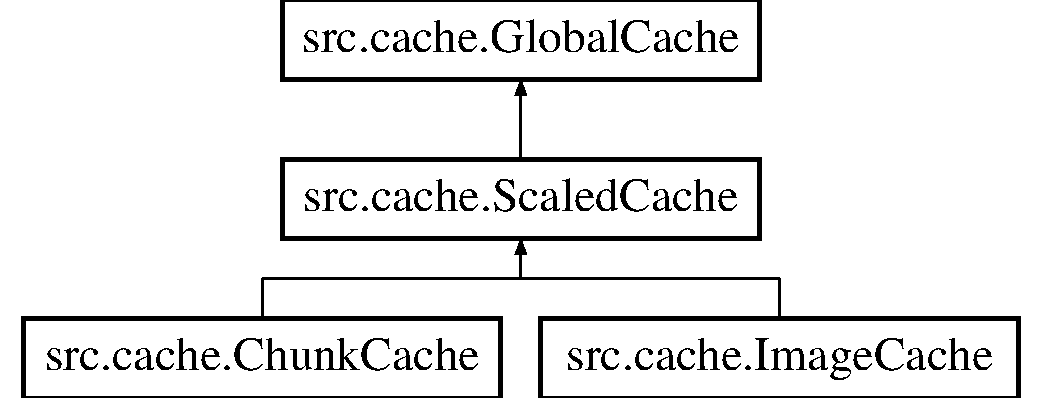
\includegraphics[height=3.000000cm]{classsrc_1_1cache_1_1_scaled_cache}
\end{center}
\end{figure}
\subsection*{\-Public \-Member \-Functions}
\begin{DoxyCompactItemize}
\item 
\hypertarget{classsrc_1_1cache_1_1_scaled_cache_ab5f3c86d112521b604d2550cffe91a12}{def {\bfseries add\-\_\-scaled}}\label{classsrc_1_1cache_1_1_scaled_cache_ab5f3c86d112521b604d2550cffe91a12}

\item 
\hypertarget{classsrc_1_1cache_1_1_scaled_cache_a93151f8e5cc63929e645090f7722cf75}{def {\bfseries remove}}\label{classsrc_1_1cache_1_1_scaled_cache_a93151f8e5cc63929e645090f7722cf75}

\item 
\hypertarget{classsrc_1_1cache_1_1_scaled_cache_aab73cd22bce9c3036221d2b3ae403aa6}{def {\bfseries get\-\_\-elt}}\label{classsrc_1_1cache_1_1_scaled_cache_aab73cd22bce9c3036221d2b3ae403aa6}

\item 
\hypertarget{classsrc_1_1cache_1_1_scaled_cache_a5a18613fcfe33f82cf1e592461100305}{def {\bfseries free\-\_\-cache}}\label{classsrc_1_1cache_1_1_scaled_cache_a5a18613fcfe33f82cf1e592461100305}

\end{DoxyCompactItemize}


\subsection{\-Detailed \-Description}
\begin{DoxyVerb}
Each entry in the cache is an array of the same object at
different scales.
\end{DoxyVerb}
 

\-The documentation for this class was generated from the following file\-:\begin{DoxyCompactItemize}
\item 
src/cache.\-py\end{DoxyCompactItemize}

\hypertarget{classsrc_1_1server_1_1_server}{}\section{src.\+server.\+Server Class Reference}
\label{classsrc_1_1server_1_1_server}\index{src.\+server.\+Server@{src.\+server.\+Server}}
\subsection*{Public Member Functions}
\begin{DoxyCompactItemize}
\item 
\hypertarget{classsrc_1_1server_1_1_server_a27ea9745051f704a10fd34ad245aa434}{}\label{classsrc_1_1server_1_1_server_a27ea9745051f704a10fd34ad245aa434} 
def {\bfseries \+\_\+\+\_\+init\+\_\+\+\_\+} (self, path)
\item 
\hypertarget{classsrc_1_1server_1_1_server_ac0c681fd1c348e0264de78a8e10ceb72}{}\label{classsrc_1_1server_1_1_server_ac0c681fd1c348e0264de78a8e10ceb72} 
def {\bfseries \+\_\+\+\_\+del\+\_\+\+\_\+} (self)
\item 
\hypertarget{classsrc_1_1server_1_1_server_a4684dc4abbdb9872a96dfe0180a4b86a}{}\label{classsrc_1_1server_1_1_server_a4684dc4abbdb9872a96dfe0180a4b86a} 
def {\bfseries run} (self)
\item 
\hypertarget{classsrc_1_1server_1_1_server_a977b8613f70094801c988c818e83fd83}{}\label{classsrc_1_1server_1_1_server_a977b8613f70094801c988c818e83fd83} 
def {\bfseries main} (self)
\item 
\hypertarget{classsrc_1_1server_1_1_server_ac18ec25ce0de8a0984b7ba3e7f77d937}{}\label{classsrc_1_1server_1_1_server_ac18ec25ce0de8a0984b7ba3e7f77d937} 
def {\bfseries handle\+Event} (self, emitter, event)
\end{DoxyCompactItemize}
\subsection*{Public Attributes}
\begin{DoxyCompactItemize}
\item 
\hypertarget{classsrc_1_1server_1_1_server_ab2030f2ecb47bda84d60911ca3160b54}{}\label{classsrc_1_1server_1_1_server_ab2030f2ecb47bda84d60911ca3160b54} 
{\bfseries loop}
\item 
\hypertarget{classsrc_1_1server_1_1_server_ad34d86b9dcf48b265b7ad8bd900d04e5}{}\label{classsrc_1_1server_1_1_server_ad34d86b9dcf48b265b7ad8bd900d04e5} 
{\bfseries net}
\item 
\hypertarget{classsrc_1_1server_1_1_server_a5d20f9b0fe55640af8e93cb47411d64b}{}\label{classsrc_1_1server_1_1_server_a5d20f9b0fe55640af8e93cb47411d64b} 
{\bfseries world}
\item 
\hypertarget{classsrc_1_1server_1_1_server_aa21a201ebc793109dee562b6e2f6aa0e}{}\label{classsrc_1_1server_1_1_server_aa21a201ebc793109dee562b6e2f6aa0e} 
{\bfseries actions}
\item 
\hypertarget{classsrc_1_1server_1_1_server_a3e70ee05d9d5f91e81569c59da3cbce0}{}\label{classsrc_1_1server_1_1_server_a3e70ee05d9d5f91e81569c59da3cbce0} 
{\bfseries timer}
\item 
\hypertarget{classsrc_1_1server_1_1_server_abd9ce5712c56d7337132daa5b9c92994}{}\label{classsrc_1_1server_1_1_server_abd9ce5712c56d7337132daa5b9c92994} 
{\bfseries order\+Dispatcher}
\item 
\hypertarget{classsrc_1_1server_1_1_server_ab9e4c5dfe23adbcd3b278b7b04c3d783}{}\label{classsrc_1_1server_1_1_server_ab9e4c5dfe23adbcd3b278b7b04c3d783} 
{\bfseries events}
\item 
\hypertarget{classsrc_1_1server_1_1_server_af27c7bccdf32aa95b87b661e4f065a49}{}\label{classsrc_1_1server_1_1_server_af27c7bccdf32aa95b87b661e4f065a49} 
{\bfseries pause}
\item 
\hypertarget{classsrc_1_1server_1_1_server_a319ab717e0d6fb53a32d68d341de5463}{}\label{classsrc_1_1server_1_1_server_a319ab717e0d6fb53a32d68d341de5463} 
{\bfseries co\+Entities}
\end{DoxyCompactItemize}


\subsection{Detailed Description}
\begin{DoxyVerb}Classe principale du processus serveur, concilie réseau, monde, actions et timer \end{DoxyVerb}
 

The documentation for this class was generated from the following file\+:\begin{DoxyCompactItemize}
\item 
src/server.\+py\end{DoxyCompactItemize}

\hypertarget{classsrc_1_1network_1_1_server_connection}{}\section{src.\+network.\+Server\+Connection Class Reference}
\label{classsrc_1_1network_1_1_server_connection}\index{src.\+network.\+Server\+Connection@{src.\+network.\+Server\+Connection}}
\subsection*{Public Member Functions}
\begin{DoxyCompactItemize}
\item 
\hypertarget{classsrc_1_1network_1_1_server_connection_aa9cb8731fc189dea188b7414f9af919d}{}\label{classsrc_1_1network_1_1_server_connection_aa9cb8731fc189dea188b7414f9af919d} 
def {\bfseries \+\_\+\+\_\+init\+\_\+\+\_\+} (self, reader, writer, handle, parent)
\item 
def \hyperlink{classsrc_1_1network_1_1_server_connection_a90815003d240ea16f574c3bb718c2fe2}{run} (self)
\item 
\hypertarget{classsrc_1_1network_1_1_server_connection_a97bdb63ff84370566329822eed5067d0}{}\label{classsrc_1_1network_1_1_server_connection_a97bdb63ff84370566329822eed5067d0} 
def {\bfseries send} (self, m)
\item 
\hypertarget{classsrc_1_1network_1_1_server_connection_a6a3b4cb4def11f7d5f8f2e154479248b}{}\label{classsrc_1_1network_1_1_server_connection_a6a3b4cb4def11f7d5f8f2e154479248b} 
def {\bfseries end} (self)
\end{DoxyCompactItemize}
\subsection*{Public Attributes}
\begin{DoxyCompactItemize}
\item 
\hypertarget{classsrc_1_1network_1_1_server_connection_a4bd50fbdebf2a26a395f6f5315fb3405}{}\label{classsrc_1_1network_1_1_server_connection_a4bd50fbdebf2a26a395f6f5315fb3405} 
{\bfseries reader}
\item 
\hypertarget{classsrc_1_1network_1_1_server_connection_aef8c4d5e35e0113fd7c75e249e469fb9}{}\label{classsrc_1_1network_1_1_server_connection_aef8c4d5e35e0113fd7c75e249e469fb9} 
{\bfseries writer}
\item 
\hypertarget{classsrc_1_1network_1_1_server_connection_a7f3534db8f1973fd35c15680c03e5c4d}{}\label{classsrc_1_1network_1_1_server_connection_a7f3534db8f1973fd35c15680c03e5c4d} 
{\bfseries handle}
\item 
\hypertarget{classsrc_1_1network_1_1_server_connection_a2422ae5d77f824318d3d90a00426bdea}{}\label{classsrc_1_1network_1_1_server_connection_a2422ae5d77f824318d3d90a00426bdea} 
{\bfseries entity}
\item 
\hypertarget{classsrc_1_1network_1_1_server_connection_acc1fdbe1f95a27cda852cb08255d5811}{}\label{classsrc_1_1network_1_1_server_connection_acc1fdbe1f95a27cda852cb08255d5811} 
{\bfseries server}
\end{DoxyCompactItemize}


\subsection{Detailed Description}
\begin{DoxyVerb}This thread manages the communications with one particular client (one
thread is created by client).
\end{DoxyVerb}
 

\subsection{Member Function Documentation}
\hypertarget{classsrc_1_1network_1_1_server_connection_a90815003d240ea16f574c3bb718c2fe2}{}\label{classsrc_1_1network_1_1_server_connection_a90815003d240ea16f574c3bb718c2fe2} 
\index{src\+::network\+::\+Server\+Connection@{src\+::network\+::\+Server\+Connection}!run@{run}}
\index{run@{run}!src\+::network\+::\+Server\+Connection@{src\+::network\+::\+Server\+Connection}}
\subsubsection{\texorpdfstring{run()}{run()}}
{\footnotesize\ttfamily def src.\+network.\+Server\+Connection.\+run (\begin{DoxyParamCaption}\item[{}]{self }\end{DoxyParamCaption})}

\begin{DoxyVerb}Wait for messages from the client and handle them immediately.
\end{DoxyVerb}
 

The documentation for this class was generated from the following file\+:\begin{DoxyCompactItemize}
\item 
src/network.\+py\end{DoxyCompactItemize}

\hypertarget{classsrc_1_1tools_1_1_timer}{}\section{src.\+tools.\+Timer Class Reference}
\label{classsrc_1_1tools_1_1_timer}\index{src.\+tools.\+Timer@{src.\+tools.\+Timer}}
\subsection*{Public Member Functions}
\begin{DoxyCompactItemize}
\item 
\hypertarget{classsrc_1_1tools_1_1_timer_a728bb045eaf7cbf58e8b1c332febb474}{}\label{classsrc_1_1tools_1_1_timer_a728bb045eaf7cbf58e8b1c332febb474} 
def {\bfseries \+\_\+\+\_\+init\+\_\+\+\_\+} (self, time\+Func=time)
\item 
def \hyperlink{classsrc_1_1tools_1_1_timer_a9aed0346c5a6131bb4cc02821f11ad73}{add} (self, time, func, args)
\item 
\hypertarget{classsrc_1_1tools_1_1_timer_a8ee9a8b99ee0a07c6ba3abea81256f0e}{}\label{classsrc_1_1tools_1_1_timer_a8ee9a8b99ee0a07c6ba3abea81256f0e} 
def {\bfseries run} (self)
\end{DoxyCompactItemize}
\subsection*{Public Attributes}
\begin{DoxyCompactItemize}
\item 
\hypertarget{classsrc_1_1tools_1_1_timer_a350e9e0548e5b28198dd3c1a4e7f03dc}{}\label{classsrc_1_1tools_1_1_timer_a350e9e0548e5b28198dd3c1a4e7f03dc} 
{\bfseries dt}
\item 
\hypertarget{classsrc_1_1tools_1_1_timer_a20a7f3faab76ac0e0668d9dcb3ccbef0}{}\label{classsrc_1_1tools_1_1_timer_a20a7f3faab76ac0e0668d9dcb3ccbef0} 
{\bfseries step}
\item 
\hypertarget{classsrc_1_1tools_1_1_timer_aca5fc0fd4c4e48f152c44a7412329dd5}{}\label{classsrc_1_1tools_1_1_timer_aca5fc0fd4c4e48f152c44a7412329dd5} 
{\bfseries heap}
\item 
\hypertarget{classsrc_1_1tools_1_1_timer_afc0baeda820a2c7c90cc0997cefbd8e6}{}\label{classsrc_1_1tools_1_1_timer_afc0baeda820a2c7c90cc0997cefbd8e6} 
{\bfseries pause}
\item 
\hypertarget{classsrc_1_1tools_1_1_timer_aa03005bc66f5e7ef870e3f016be07111}{}\label{classsrc_1_1tools_1_1_timer_aa03005bc66f5e7ef870e3f016be07111} 
{\bfseries count}
\item 
\hypertarget{classsrc_1_1tools_1_1_timer_adf4d5c3f24b07c38d18ef5470af52d93}{}\label{classsrc_1_1tools_1_1_timer_adf4d5c3f24b07c38d18ef5470af52d93} 
{\bfseries time}
\end{DoxyCompactItemize}


\subsection{Detailed Description}
\begin{DoxyVerb}Déclenche des appels différés de couroutine \end{DoxyVerb}
 

\subsection{Member Function Documentation}
\hypertarget{classsrc_1_1tools_1_1_timer_a9aed0346c5a6131bb4cc02821f11ad73}{}\label{classsrc_1_1tools_1_1_timer_a9aed0346c5a6131bb4cc02821f11ad73} 
\index{src\+::tools\+::\+Timer@{src\+::tools\+::\+Timer}!add@{add}}
\index{add@{add}!src\+::tools\+::\+Timer@{src\+::tools\+::\+Timer}}
\subsubsection{\texorpdfstring{add()}{add()}}
{\footnotesize\ttfamily def src.\+tools.\+Timer.\+add (\begin{DoxyParamCaption}\item[{}]{self,  }\item[{}]{time,  }\item[{}]{func,  }\item[{}]{args }\end{DoxyParamCaption})}

\begin{DoxyVerb}Inscrit l'appel de func avec les arguments args \end{DoxyVerb}
 

The documentation for this class was generated from the following file\+:\begin{DoxyCompactItemize}
\item 
src/tools.\+py\end{DoxyCompactItemize}

\hypertarget{classsrc_1_1utils_1_1_walkable_graph}{\section{src.\-utils.\-Walkable\-Graph \-Class \-Reference}
\label{classsrc_1_1utils_1_1_walkable_graph}\index{src.\-utils.\-Walkable\-Graph@{src.\-utils.\-Walkable\-Graph}}
}
\subsection*{\-Public \-Member \-Functions}
\begin{DoxyCompactItemize}
\item 
def \hyperlink{classsrc_1_1utils_1_1_walkable_graph_a61fad39577edd7672f9ff090ed8be884}{\-\_\-\-\_\-init\-\_\-\-\_\-}
\item 
def \hyperlink{classsrc_1_1utils_1_1_walkable_graph_a209beb8622e9c2fb742c6cbc77071d68}{get\-\_\-neighbors}
\item 
def \hyperlink{classsrc_1_1utils_1_1_walkable_graph_ab4f469cf0e73b91cd576d9526795ff70}{dist}
\item 
def \hyperlink{classsrc_1_1utils_1_1_walkable_graph_ae4a3c59b8bef04194e4f92f2e8f2b06b}{get\-\_\-path}
\end{DoxyCompactItemize}
\subsection*{\-Public \-Attributes}
\begin{DoxyCompactItemize}
\item 
\hypertarget{classsrc_1_1utils_1_1_walkable_graph_a1df908d75835d45e9304bc698186bbec}{{\bfseries walkables}}\label{classsrc_1_1utils_1_1_walkable_graph_a1df908d75835d45e9304bc698186bbec}

\end{DoxyCompactItemize}


\subsection{\-Constructor \& \-Destructor \-Documentation}
\hypertarget{classsrc_1_1utils_1_1_walkable_graph_a61fad39577edd7672f9ff090ed8be884}{\index{src\-::utils\-::\-Walkable\-Graph@{src\-::utils\-::\-Walkable\-Graph}!\-\_\-\-\_\-init\-\_\-\-\_\-@{\-\_\-\-\_\-init\-\_\-\-\_\-}}
\index{\-\_\-\-\_\-init\-\_\-\-\_\-@{\-\_\-\-\_\-init\-\_\-\-\_\-}!src::utils::WalkableGraph@{src\-::utils\-::\-Walkable\-Graph}}
\subsubsection[{\-\_\-\-\_\-init\-\_\-\-\_\-}]{\setlength{\rightskip}{0pt plus 5cm}def {\bf src.\-utils.\-Walkable\-Graph.\-\_\-\-\_\-init\-\_\-\-\_\-} (
\begin{DoxyParamCaption}
\item[{}]{self, }
\item[{}]{walkables}
\end{DoxyParamCaption}
)}}\label{classsrc_1_1utils_1_1_walkable_graph_a61fad39577edd7672f9ff090ed8be884}
\begin{DoxyVerb}
Walkables is a bit array representing cells that can be crossed
during a move
\end{DoxyVerb}
 

\subsection{\-Member \-Function \-Documentation}
\hypertarget{classsrc_1_1utils_1_1_walkable_graph_ab4f469cf0e73b91cd576d9526795ff70}{\index{src\-::utils\-::\-Walkable\-Graph@{src\-::utils\-::\-Walkable\-Graph}!dist@{dist}}
\index{dist@{dist}!src::utils::WalkableGraph@{src\-::utils\-::\-Walkable\-Graph}}
\subsubsection[{dist}]{\setlength{\rightskip}{0pt plus 5cm}def {\bf src.\-utils.\-Walkable\-Graph.\-dist} (
\begin{DoxyParamCaption}
\item[{}]{self, }
\item[{}]{u, }
\item[{}]{v}
\end{DoxyParamCaption}
)}}\label{classsrc_1_1utils_1_1_walkable_graph_ab4f469cf0e73b91cd576d9526795ff70}
\begin{DoxyVerb}Return distance between two nodes on the grid \end{DoxyVerb}
 \hypertarget{classsrc_1_1utils_1_1_walkable_graph_a209beb8622e9c2fb742c6cbc77071d68}{\index{src\-::utils\-::\-Walkable\-Graph@{src\-::utils\-::\-Walkable\-Graph}!get\-\_\-neighbors@{get\-\_\-neighbors}}
\index{get\-\_\-neighbors@{get\-\_\-neighbors}!src::utils::WalkableGraph@{src\-::utils\-::\-Walkable\-Graph}}
\subsubsection[{get\-\_\-neighbors}]{\setlength{\rightskip}{0pt plus 5cm}def {\bf src.\-utils.\-Walkable\-Graph.\-get\-\_\-neighbors} (
\begin{DoxyParamCaption}
\item[{}]{self, }
\item[{}]{index}
\end{DoxyParamCaption}
)}}\label{classsrc_1_1utils_1_1_walkable_graph_a209beb8622e9c2fb742c6cbc77071d68}
\begin{DoxyVerb}
Return accessible cells around index, with a cost value depending
on the direction of the move.
\end{DoxyVerb}
 \hypertarget{classsrc_1_1utils_1_1_walkable_graph_ae4a3c59b8bef04194e4f92f2e8f2b06b}{\index{src\-::utils\-::\-Walkable\-Graph@{src\-::utils\-::\-Walkable\-Graph}!get\-\_\-path@{get\-\_\-path}}
\index{get\-\_\-path@{get\-\_\-path}!src::utils::WalkableGraph@{src\-::utils\-::\-Walkable\-Graph}}
\subsubsection[{get\-\_\-path}]{\setlength{\rightskip}{0pt plus 5cm}def {\bf src.\-utils.\-Walkable\-Graph.\-get\-\_\-path} (
\begin{DoxyParamCaption}
\item[{}]{self, }
\item[{}]{source, }
\item[{}]{dest}
\end{DoxyParamCaption}
)}}\label{classsrc_1_1utils_1_1_walkable_graph_ae4a3c59b8bef04194e4f92f2e8f2b06b}
\begin{DoxyVerb}A* algorithm on the current graph \end{DoxyVerb}
 

\-The documentation for this class was generated from the following file\-:\begin{DoxyCompactItemize}
\item 
src/utils.\-py\end{DoxyCompactItemize}

\hypertarget{classsrc_1_1world_1_1_world}{\section{src.\-world.\-World \-Class \-Reference}
\label{classsrc_1_1world_1_1_world}\index{src.\-world.\-World@{src.\-world.\-World}}
}
\subsection*{\-Public \-Member \-Functions}
\begin{DoxyCompactItemize}
\item 
\hypertarget{classsrc_1_1world_1_1_world_a6dea64e86406f597719dc713269c576f}{def {\bfseries \-\_\-\-\_\-init\-\_\-\-\_\-}}\label{classsrc_1_1world_1_1_world_a6dea64e86406f597719dc713269c576f}

\end{DoxyCompactItemize}
\subsection*{\-Public \-Attributes}
\begin{DoxyCompactItemize}
\item 
\hypertarget{classsrc_1_1world_1_1_world_a3d59efedb025f0fe4474071e99ff1548}{{\bfseries maps}}\label{classsrc_1_1world_1_1_world_a3d59efedb025f0fe4474071e99ff1548}

\item 
\hypertarget{classsrc_1_1world_1_1_world_a08fc5ac30d6e377914055a1688aa141f}{{\bfseries entities}}\label{classsrc_1_1world_1_1_world_a08fc5ac30d6e377914055a1688aa141f}

\item 
\hypertarget{classsrc_1_1world_1_1_world_a122d24d465ff30df9b2329d8e1e131f7}{{\bfseries objects}}\label{classsrc_1_1world_1_1_world_a122d24d465ff30df9b2329d8e1e131f7}

\end{DoxyCompactItemize}


\-The documentation for this class was generated from the following file\-:\begin{DoxyCompactItemize}
\item 
src/world.\-py\end{DoxyCompactItemize}

\hypertarget{classsrc_1_1print_world_1_1_world_viewer}{\section{src.\-print\-World.\-World\-Viewer \-Class \-Reference}
\label{classsrc_1_1print_world_1_1_world_viewer}\index{src.\-print\-World.\-World\-Viewer@{src.\-print\-World.\-World\-Viewer}}
}
\-Inheritance diagram for src.\-print\-World.\-World\-Viewer\-:\begin{figure}[H]
\begin{center}
\leavevmode
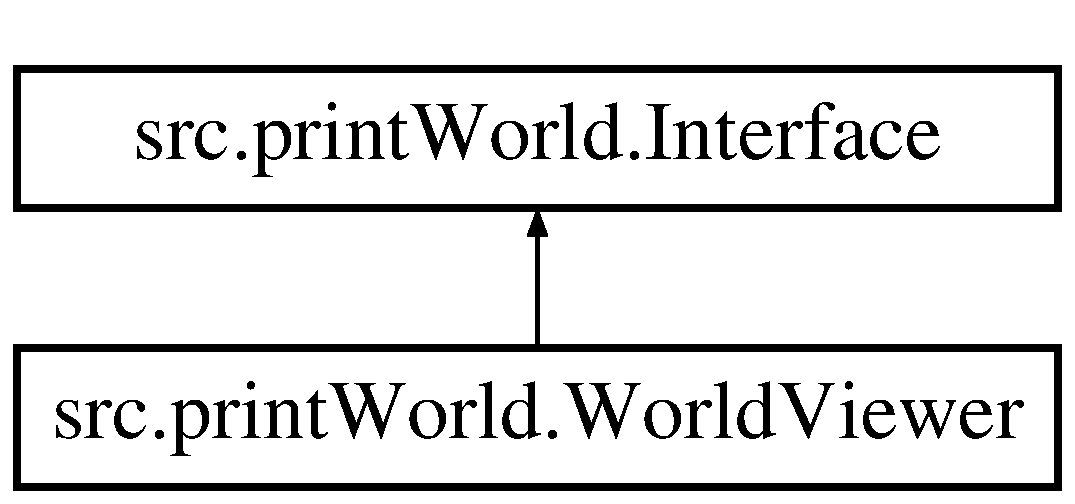
\includegraphics[height=2.000000cm]{classsrc_1_1print_world_1_1_world_viewer}
\end{center}
\end{figure}
\subsection*{\-Public \-Member \-Functions}
\begin{DoxyCompactItemize}
\item 
\hypertarget{classsrc_1_1print_world_1_1_world_viewer_a7a2696805539e858a95ee4cf45eaf1c7}{def {\bfseries \-\_\-\-\_\-init\-\_\-\-\_\-}}\label{classsrc_1_1print_world_1_1_world_viewer_a7a2696805539e858a95ee4cf45eaf1c7}

\item 
\hypertarget{classsrc_1_1print_world_1_1_world_viewer_a13a6b8596015312e1fde150640ac542e}{def {\bfseries get\-\_\-event}}\label{classsrc_1_1print_world_1_1_world_viewer_a13a6b8596015312e1fde150640ac542e}

\item 
\hypertarget{classsrc_1_1print_world_1_1_world_viewer_a1c80356e21e257f8a9f6f123b1c9970d}{def {\bfseries end}}\label{classsrc_1_1print_world_1_1_world_viewer_a1c80356e21e257f8a9f6f123b1c9970d}

\item 
\hypertarget{classsrc_1_1print_world_1_1_world_viewer_aa39257d89f22103040677719c3f8e90e}{def {\bfseries update}}\label{classsrc_1_1print_world_1_1_world_viewer_aa39257d89f22103040677719c3f8e90e}

\item 
\hypertarget{classsrc_1_1print_world_1_1_world_viewer_a6bf228bb9cd15d34ef19c624fdc79c68}{def {\bfseries render}}\label{classsrc_1_1print_world_1_1_world_viewer_a6bf228bb9cd15d34ef19c624fdc79c68}

\item 
\hypertarget{classsrc_1_1print_world_1_1_world_viewer_a4f40dfbf0e262ffbe723900a2f5cbe4f}{def {\bfseries move}}\label{classsrc_1_1print_world_1_1_world_viewer_a4f40dfbf0e262ffbe723900a2f5cbe4f}

\item 
\hypertarget{classsrc_1_1print_world_1_1_world_viewer_a552043b414d6eab1d78d2816c06f81af}{def {\bfseries zoom}}\label{classsrc_1_1print_world_1_1_world_viewer_a552043b414d6eab1d78d2816c06f81af}

\item 
\hypertarget{classsrc_1_1print_world_1_1_world_viewer_ae16b4b78785490c05644cd54fa2fd88a}{def {\bfseries move\-\_\-char}}\label{classsrc_1_1print_world_1_1_world_viewer_ae16b4b78785490c05644cd54fa2fd88a}

\item 
\hypertarget{classsrc_1_1print_world_1_1_world_viewer_a4126bfb1941eece5f72ecc7e7a20f4c2}{def {\bfseries propagate\-\_\-trigger}}\label{classsrc_1_1print_world_1_1_world_viewer_a4126bfb1941eece5f72ecc7e7a20f4c2}

\end{DoxyCompactItemize}
\subsection*{\-Public \-Attributes}
\begin{DoxyCompactItemize}
\item 
\hypertarget{classsrc_1_1print_world_1_1_world_viewer_a58eb9c3aa33233ad30953553903642e9}{{\bfseries screen\-\_\-size}}\label{classsrc_1_1print_world_1_1_world_viewer_a58eb9c3aa33233ad30953553903642e9}

\item 
\hypertarget{classsrc_1_1print_world_1_1_world_viewer_ad63b7bffafc5dbc2af5100572e9d4b55}{{\bfseries current\-\_\-map}}\label{classsrc_1_1print_world_1_1_world_viewer_ad63b7bffafc5dbc2af5100572e9d4b55}

\item 
\hypertarget{classsrc_1_1print_world_1_1_world_viewer_a739f8f3c05bb674678ec3ec6c475398f}{{\bfseries main\-\_\-char}}\label{classsrc_1_1print_world_1_1_world_viewer_a739f8f3c05bb674678ec3ec6c475398f}

\item 
\hypertarget{classsrc_1_1print_world_1_1_world_viewer_a2a7a6e13cd7009be159a91f32804dedf}{{\bfseries characters}}\label{classsrc_1_1print_world_1_1_world_viewer_a2a7a6e13cd7009be159a91f32804dedf}

\end{DoxyCompactItemize}


\-The documentation for this class was generated from the following file\-:\begin{DoxyCompactItemize}
\item 
src/print\-World.\-py\end{DoxyCompactItemize}

\printindex
\end{document}
